% Digital Logic Report Template
% Created: 2020-01-10, John Miller

%==========================================================
%=========== Document Setup  ==============================

% Formatting defined by class file
\documentclass[11pt]{article}

% ---- Document formatting ----
\usepackage[margin=1in]{geometry}	% Narrower margins
\usepackage{booktabs}				% Nice formatting of tables
\usepackage{graphicx}				% Ability to include graphics

%\setlength\parindent{0pt}	% Do not indent first line of paragraphs 
\usepackage[parfill]{parskip}		% Line space b/w paragraphs
%	parfill option prevents last line of pgrph from being fully justified

% Parskip package adds too much space around titles, fix with this
\RequirePackage{titlesec}
\titlespacing\section{0pt}{8pt plus 4pt minus 2pt}{3pt plus 2pt minus 2pt}
\titlespacing\subsection{0pt}{4pt plus 4pt minus 2pt}{-2pt plus 2pt minus 2pt}
\titlespacing\subsubsection{0pt}{2pt plus 4pt minus 2pt}{-6pt plus 2pt minus 2pt}

% ---- Hyperlinks ----
\usepackage[colorlinks=true,urlcolor=blue]{hyperref}	% For URL's. Automatically links internal references.

% ---- Code listings ----
\usepackage{listings} 					% Nice code layout and inclusion
\usepackage[usenames,dvipsnames]{xcolor}	% Colors (needs to be defined before using colors)

% Define custom colors for listings
\definecolor{listinggray}{gray}{0.98}		% Listings background color
\definecolor{rulegray}{gray}{0.7}			% Listings rule/frame color

% Style for Verilog
\lstdefinestyle{Verilog}{
	language=Verilog,					% Verilog
	backgroundcolor=\color{listinggray},	% light gray background
	rulecolor=\color{blue}, 			% blue frame lines
	frame=tb,							% lines above & below
	linewidth=\columnwidth, 			% set line width
	basicstyle=\small\ttfamily,	% basic font style that is used for the code	
	breaklines=true, 					% allow breaking across columns/pages
	tabsize=3,							% set tab size
	commentstyle=\color{gray},	% comments in italic 
	stringstyle=\upshape,				% strings are printed in normal font
	showspaces=false,					% don't underscore spaces
}

% How to use: \Verilog[listing_options]{file}
\newcommand{\Verilog}[2][]{%
	\lstinputlisting[style=Verilog,#1]{#2}
}




%======================================================
%=========== Body  ====================================
\begin{document}

\title{ELC 2137 Lab 9: Lab 9 ALU with Input Register}
\author{Makenna Meyers}

\maketitle


\section*{Summary}
 This lab incorporates registers and an Arithmetic Logic Unit (ALU) to build a small calculator. The code used can be found in Listings \ref{code:register}, \ref{code:register_test}, \ref{code:alu}, \ref{code:alu_test}, and \ref{code:top_module}, and examples of the calculator use can be found in Figures \ref{fig:add_step_1} through \ref{fig:xor_step_3}.


\section*{Results}

\begin{table*}[ht]\centering
	\caption{\textit{register} expected results table}
	\label{ALU:tbl:register_ERT}\medskip
	\begin{tabular}{l|rrrrrrrrrrr}
		Time (ns): & 0-5 & 5-10 & 10-15 & 15-20 & 20-25 & 25-30 & 30-35 & 35-40 & 40-45 & 45-50 & 50-55 \\
		\midrule
		D (hex) & 0 & 0 	  & A & A & 3 	    & 3 	  & 0 	    & 0 & 0$\to$6 & 6 & 6 \\
		clk     & 0 & 1 	  & 0 & 1 & 0 	    & 1 	  & 0 	    & 1 & 0 	  & 1 & 0 \\
		en  	& 0 & 0 	  & 1 & 1 & 1$\to$0 & 0$\to$1 & 1$\to$0 & 0 & 0$\to$1 & 1 & 1 \\
		rst 	& 0 & 0$\to$1 & 0 & 0 & 0 		& 0 	  & 0		& 0 & 0		  & 0 & 0 \\
		\midrule
		Q (hex) & X & X$\to$0 & 0 & A & A & A & A & A & A & 6 & 6 \\
		\bottomrule
	\end{tabular}
\end{table*}

\begin{table*}[ht]\centering
	\caption{\textit{alu} expected results table}
	\label{ALU:tbl:alu_ERT}\medskip
	\begin{tabular}{l|rrrrrr}
		Time (ns): & 0-10 & 10-20 & 20-30 & 30-40 & 40-50 & 50-60 \\
		\midrule
		in0 & 1 & 3 & 5 & 1 & 1 & 8 \\
		in1 & 2 & 1 & 7 & 1 & 1 & 6 \\
		op	& 0 & 1 & 2 & 3 & 4 & 5 \\
		\midrule
		out & 3 & 2 & 5 & 1 & 0 & 8 \\
		\bottomrule
	\end{tabular}
\end{table*}


\begin{figure}[ht]\centering
	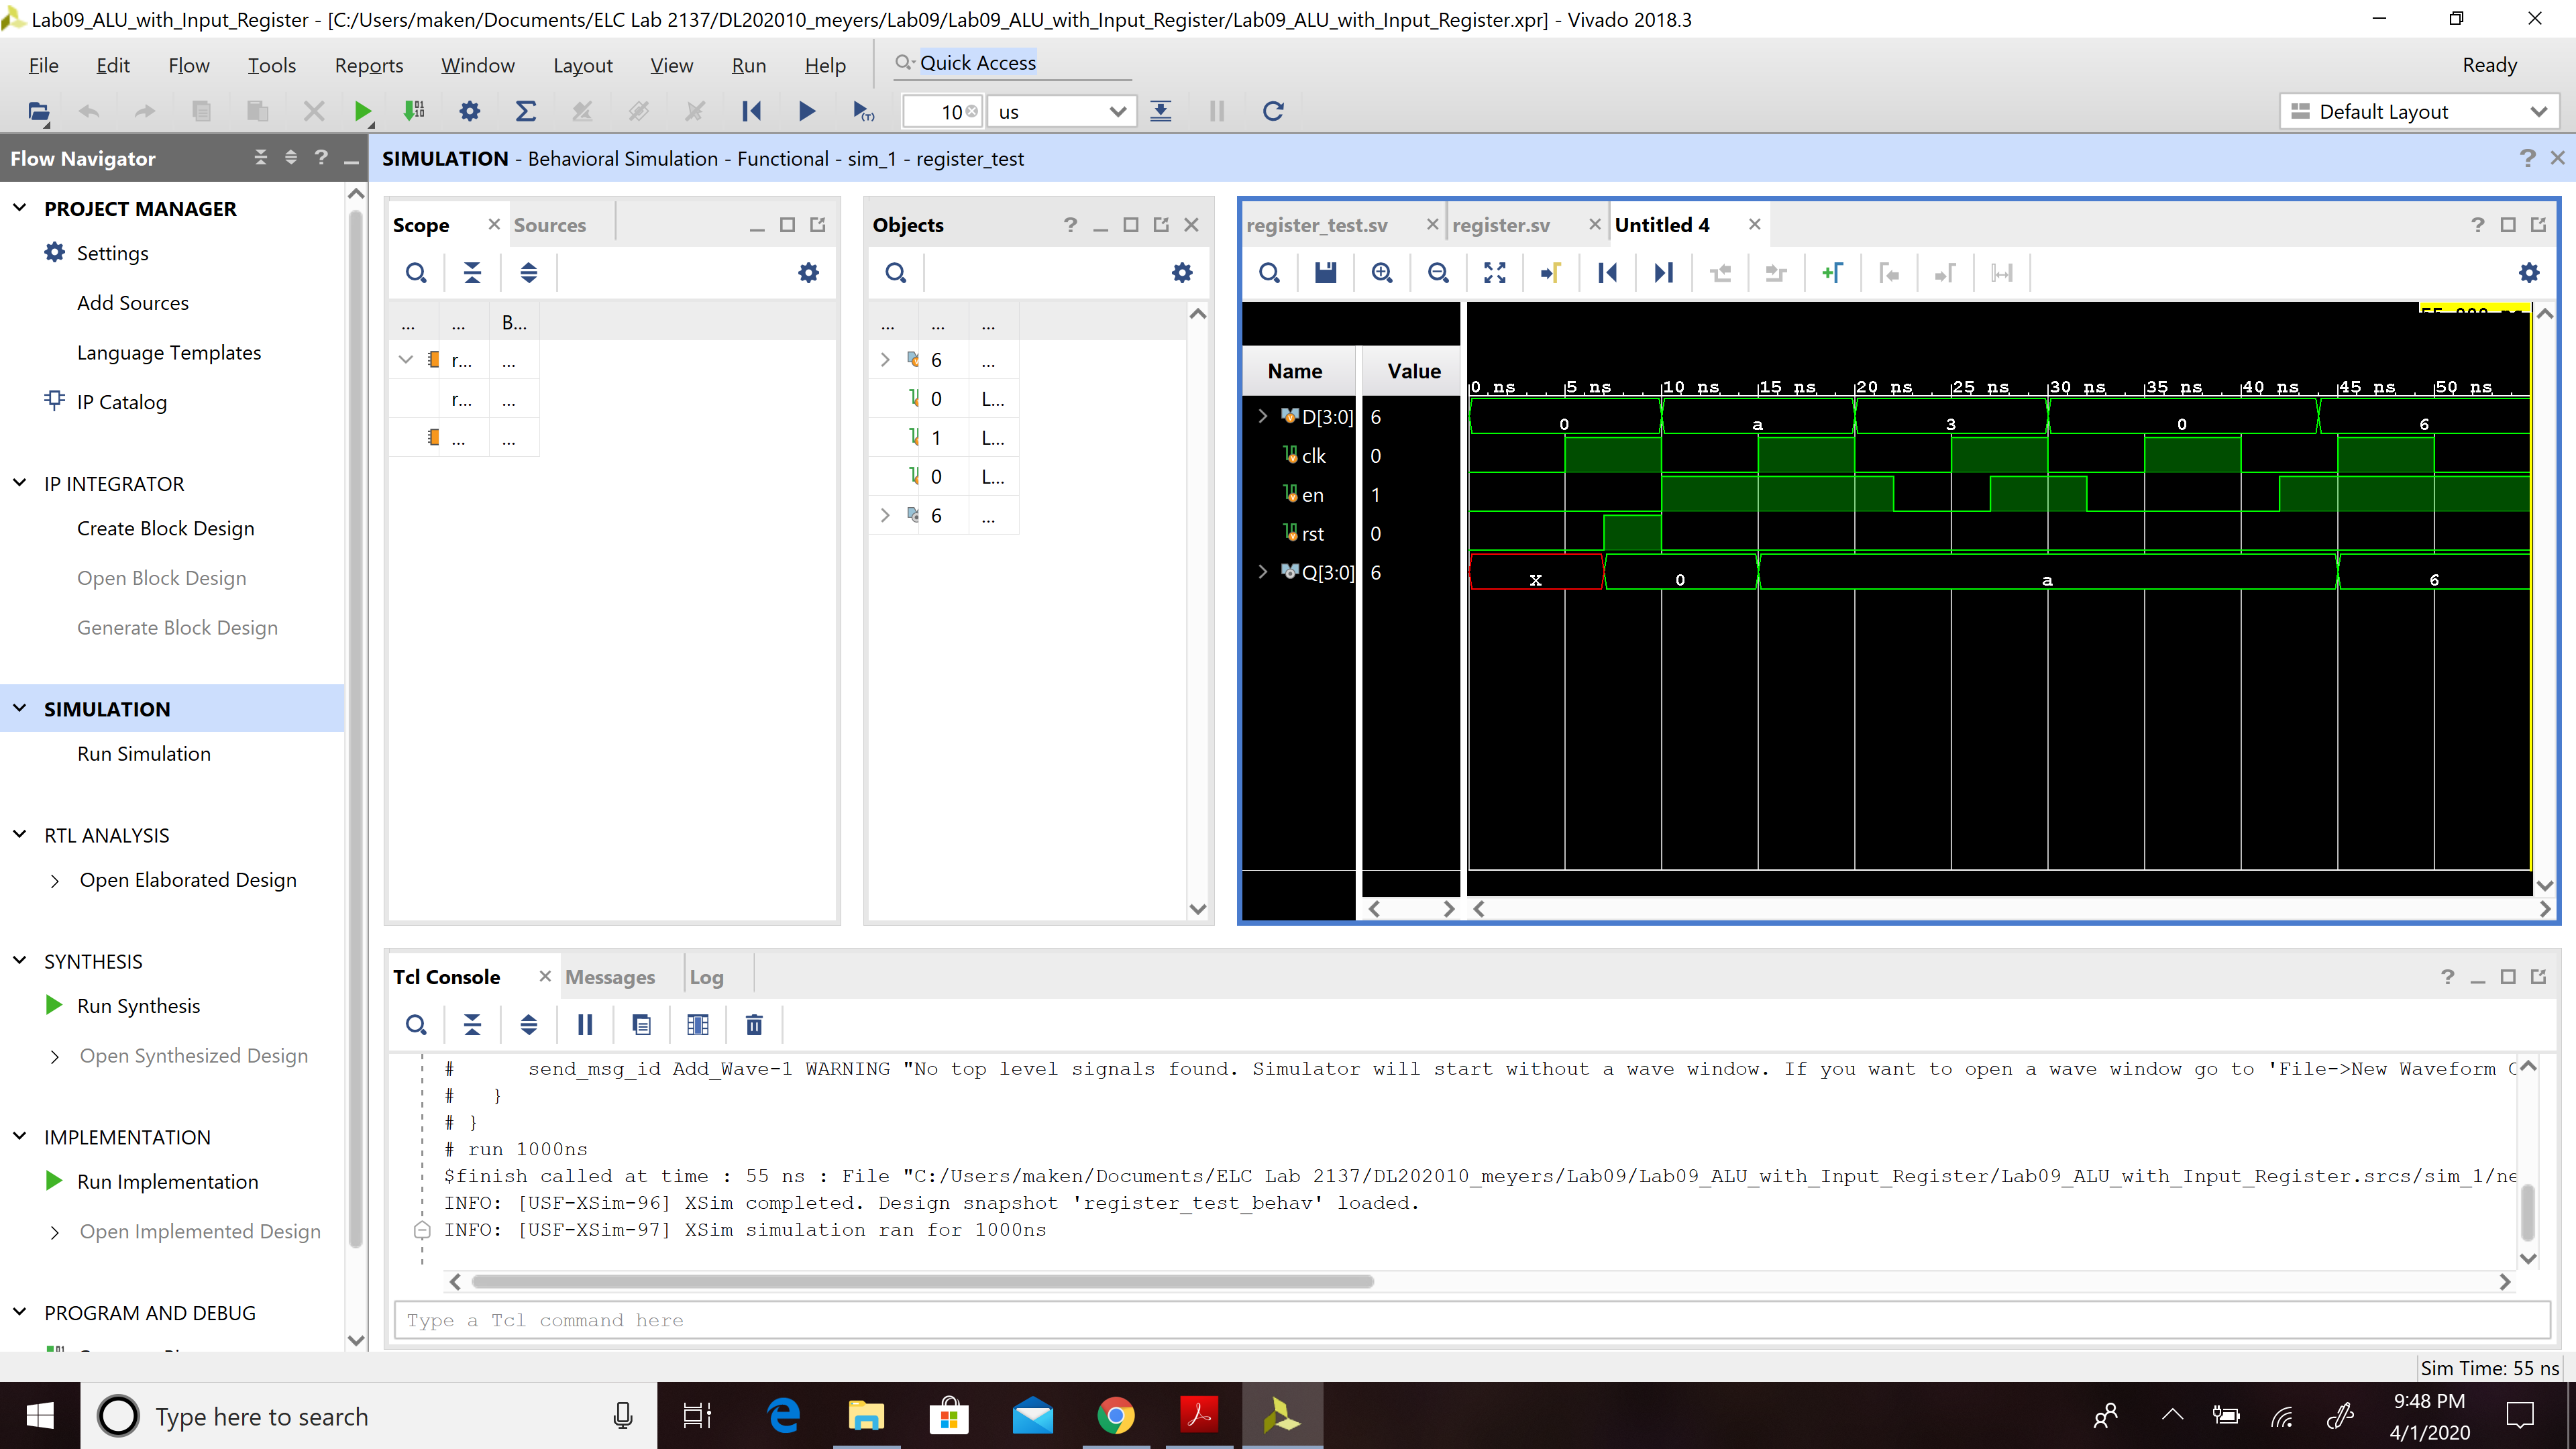
\includegraphics[width=0.8\textwidth,trim=19.5cm 12cm 0.6cm 4.8cm,clip]{register_test_screenshot}
	\caption{Register Simulation Waveform}
	\label{fig:register_sim_wave_Screenshot}			
\end{figure}

\begin{figure}[ht]\centering
	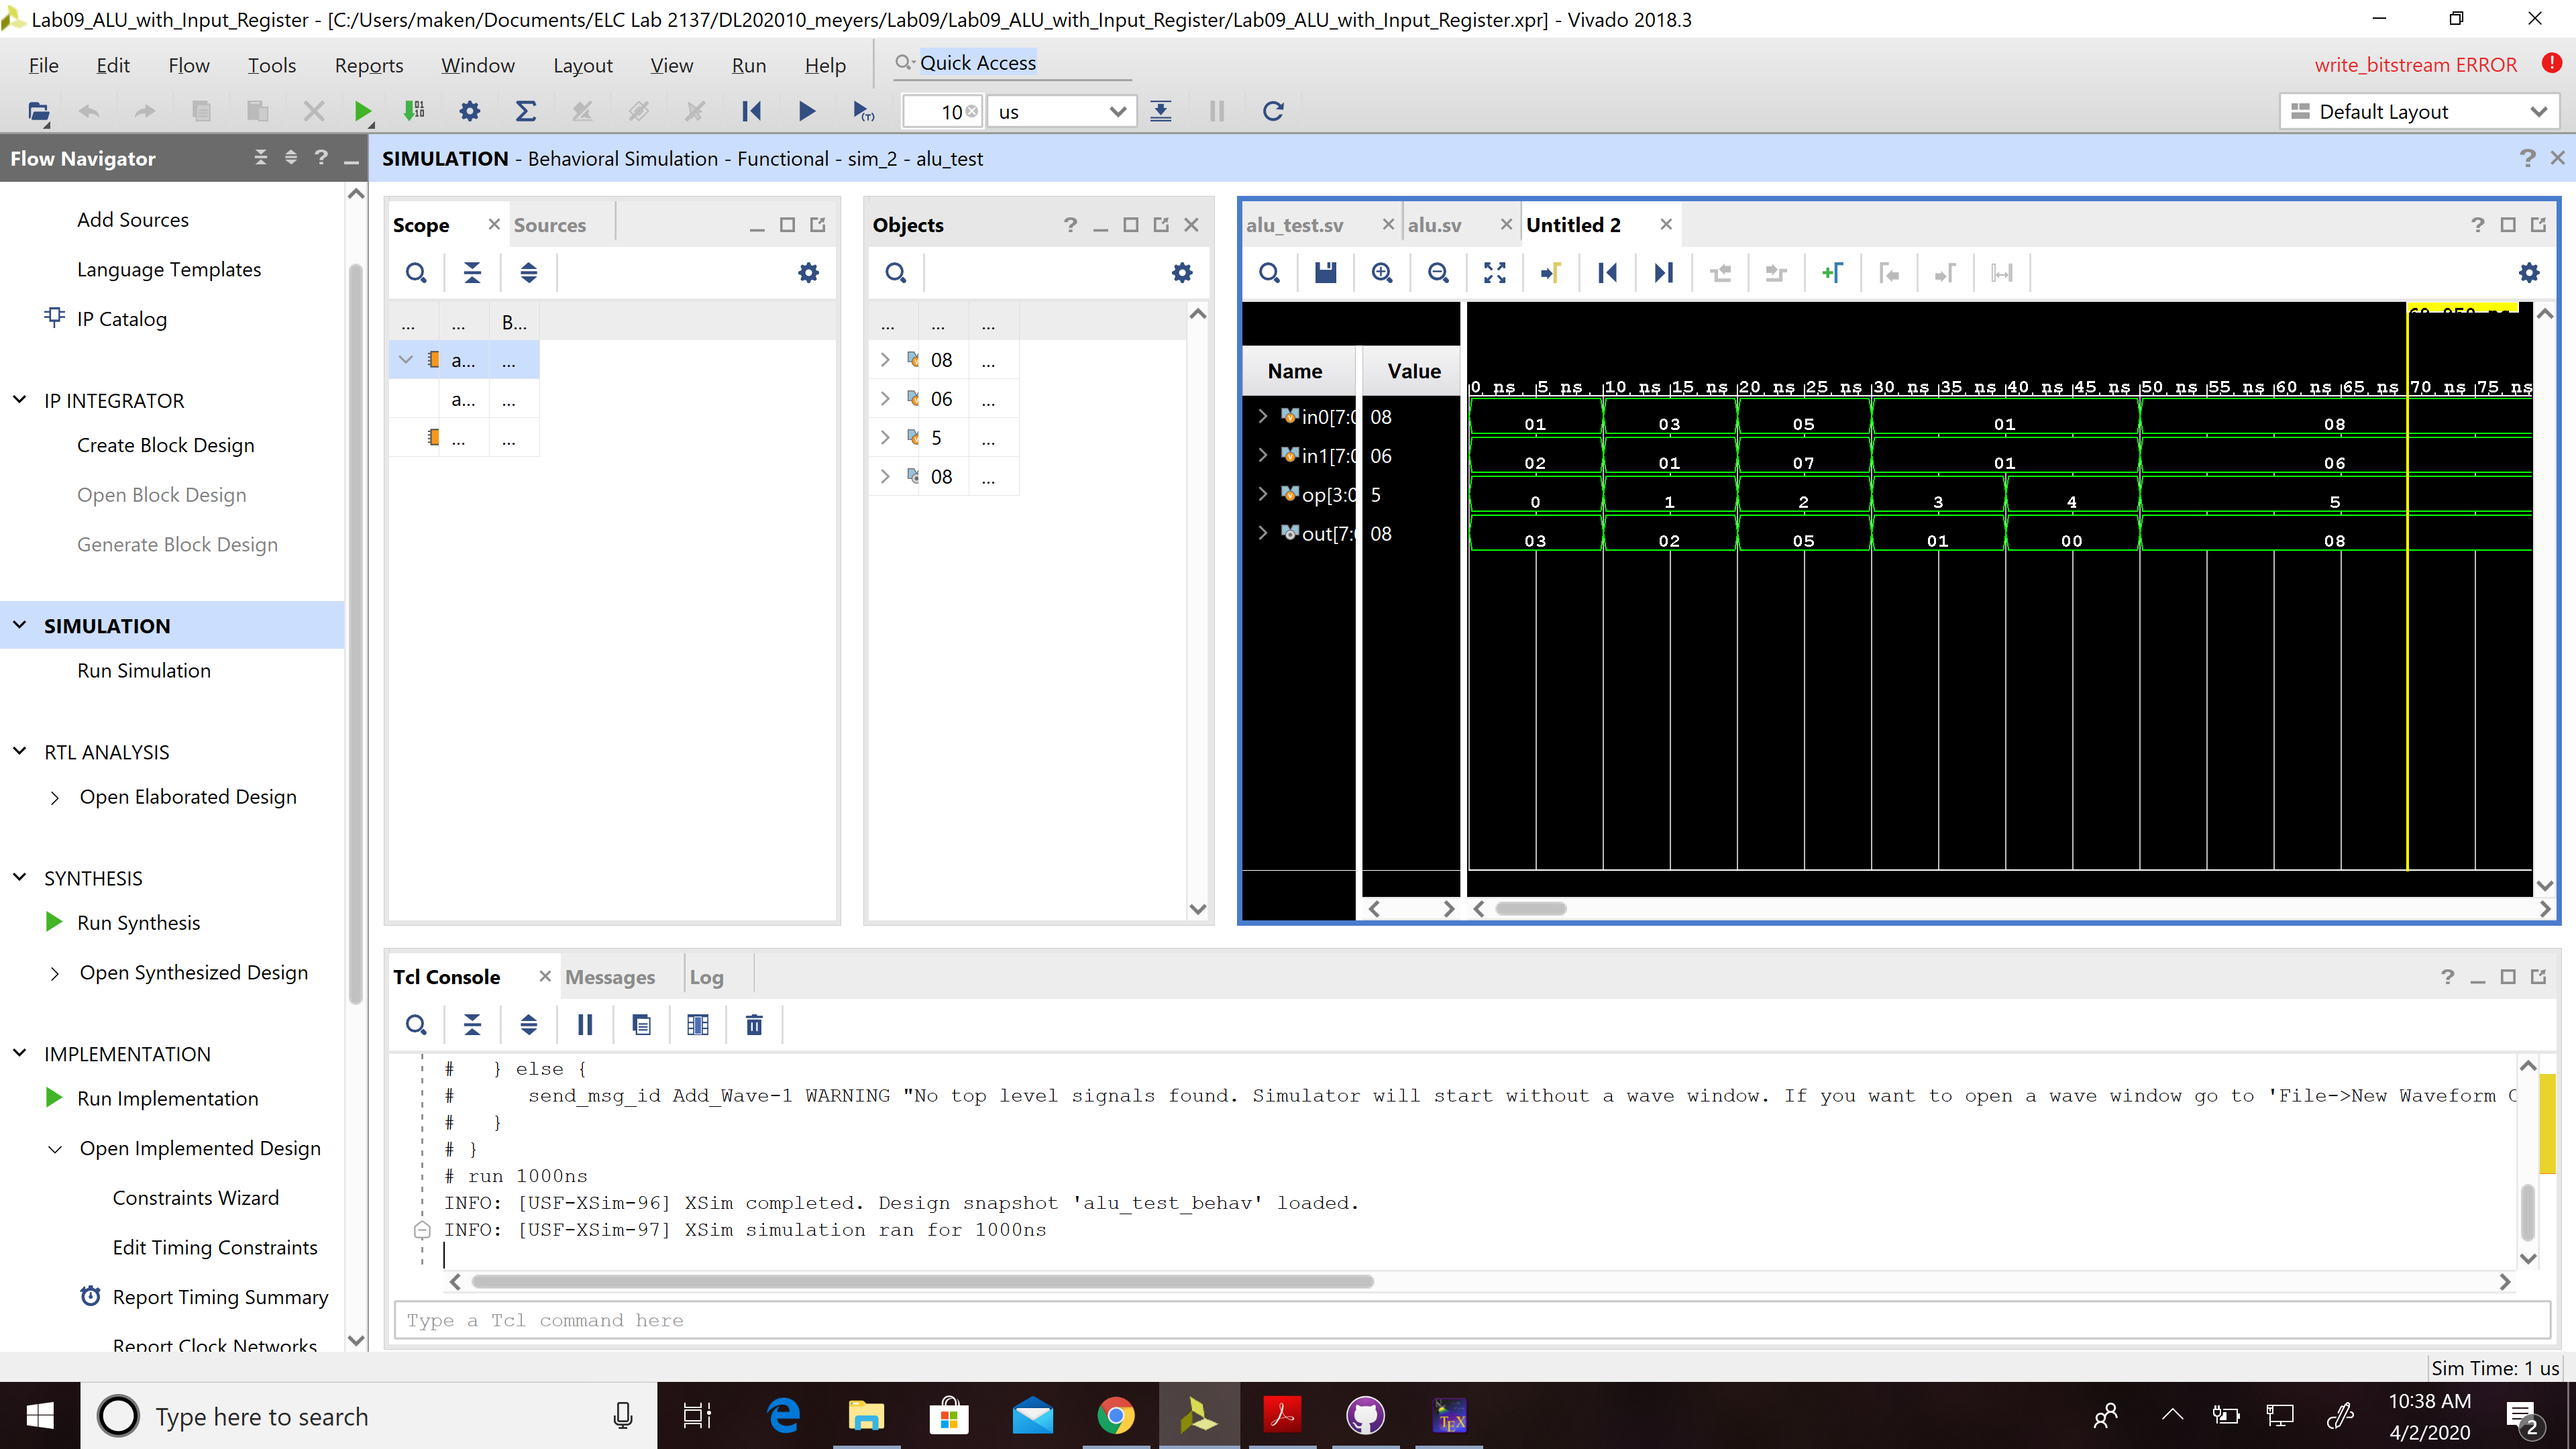
\includegraphics[width=0.8\textwidth,trim=19.5cm 12cm 3cm 4.8cm,clip]{alu_test_screenshot(1)}
	\caption{ALU Simulation Waveform}
	\label{fig:alu_sim_wave_Screenshot}			
\end{figure}
\clearpage 

\section*{Op 0: ADD}

\begin{figure}[ht]\centering
	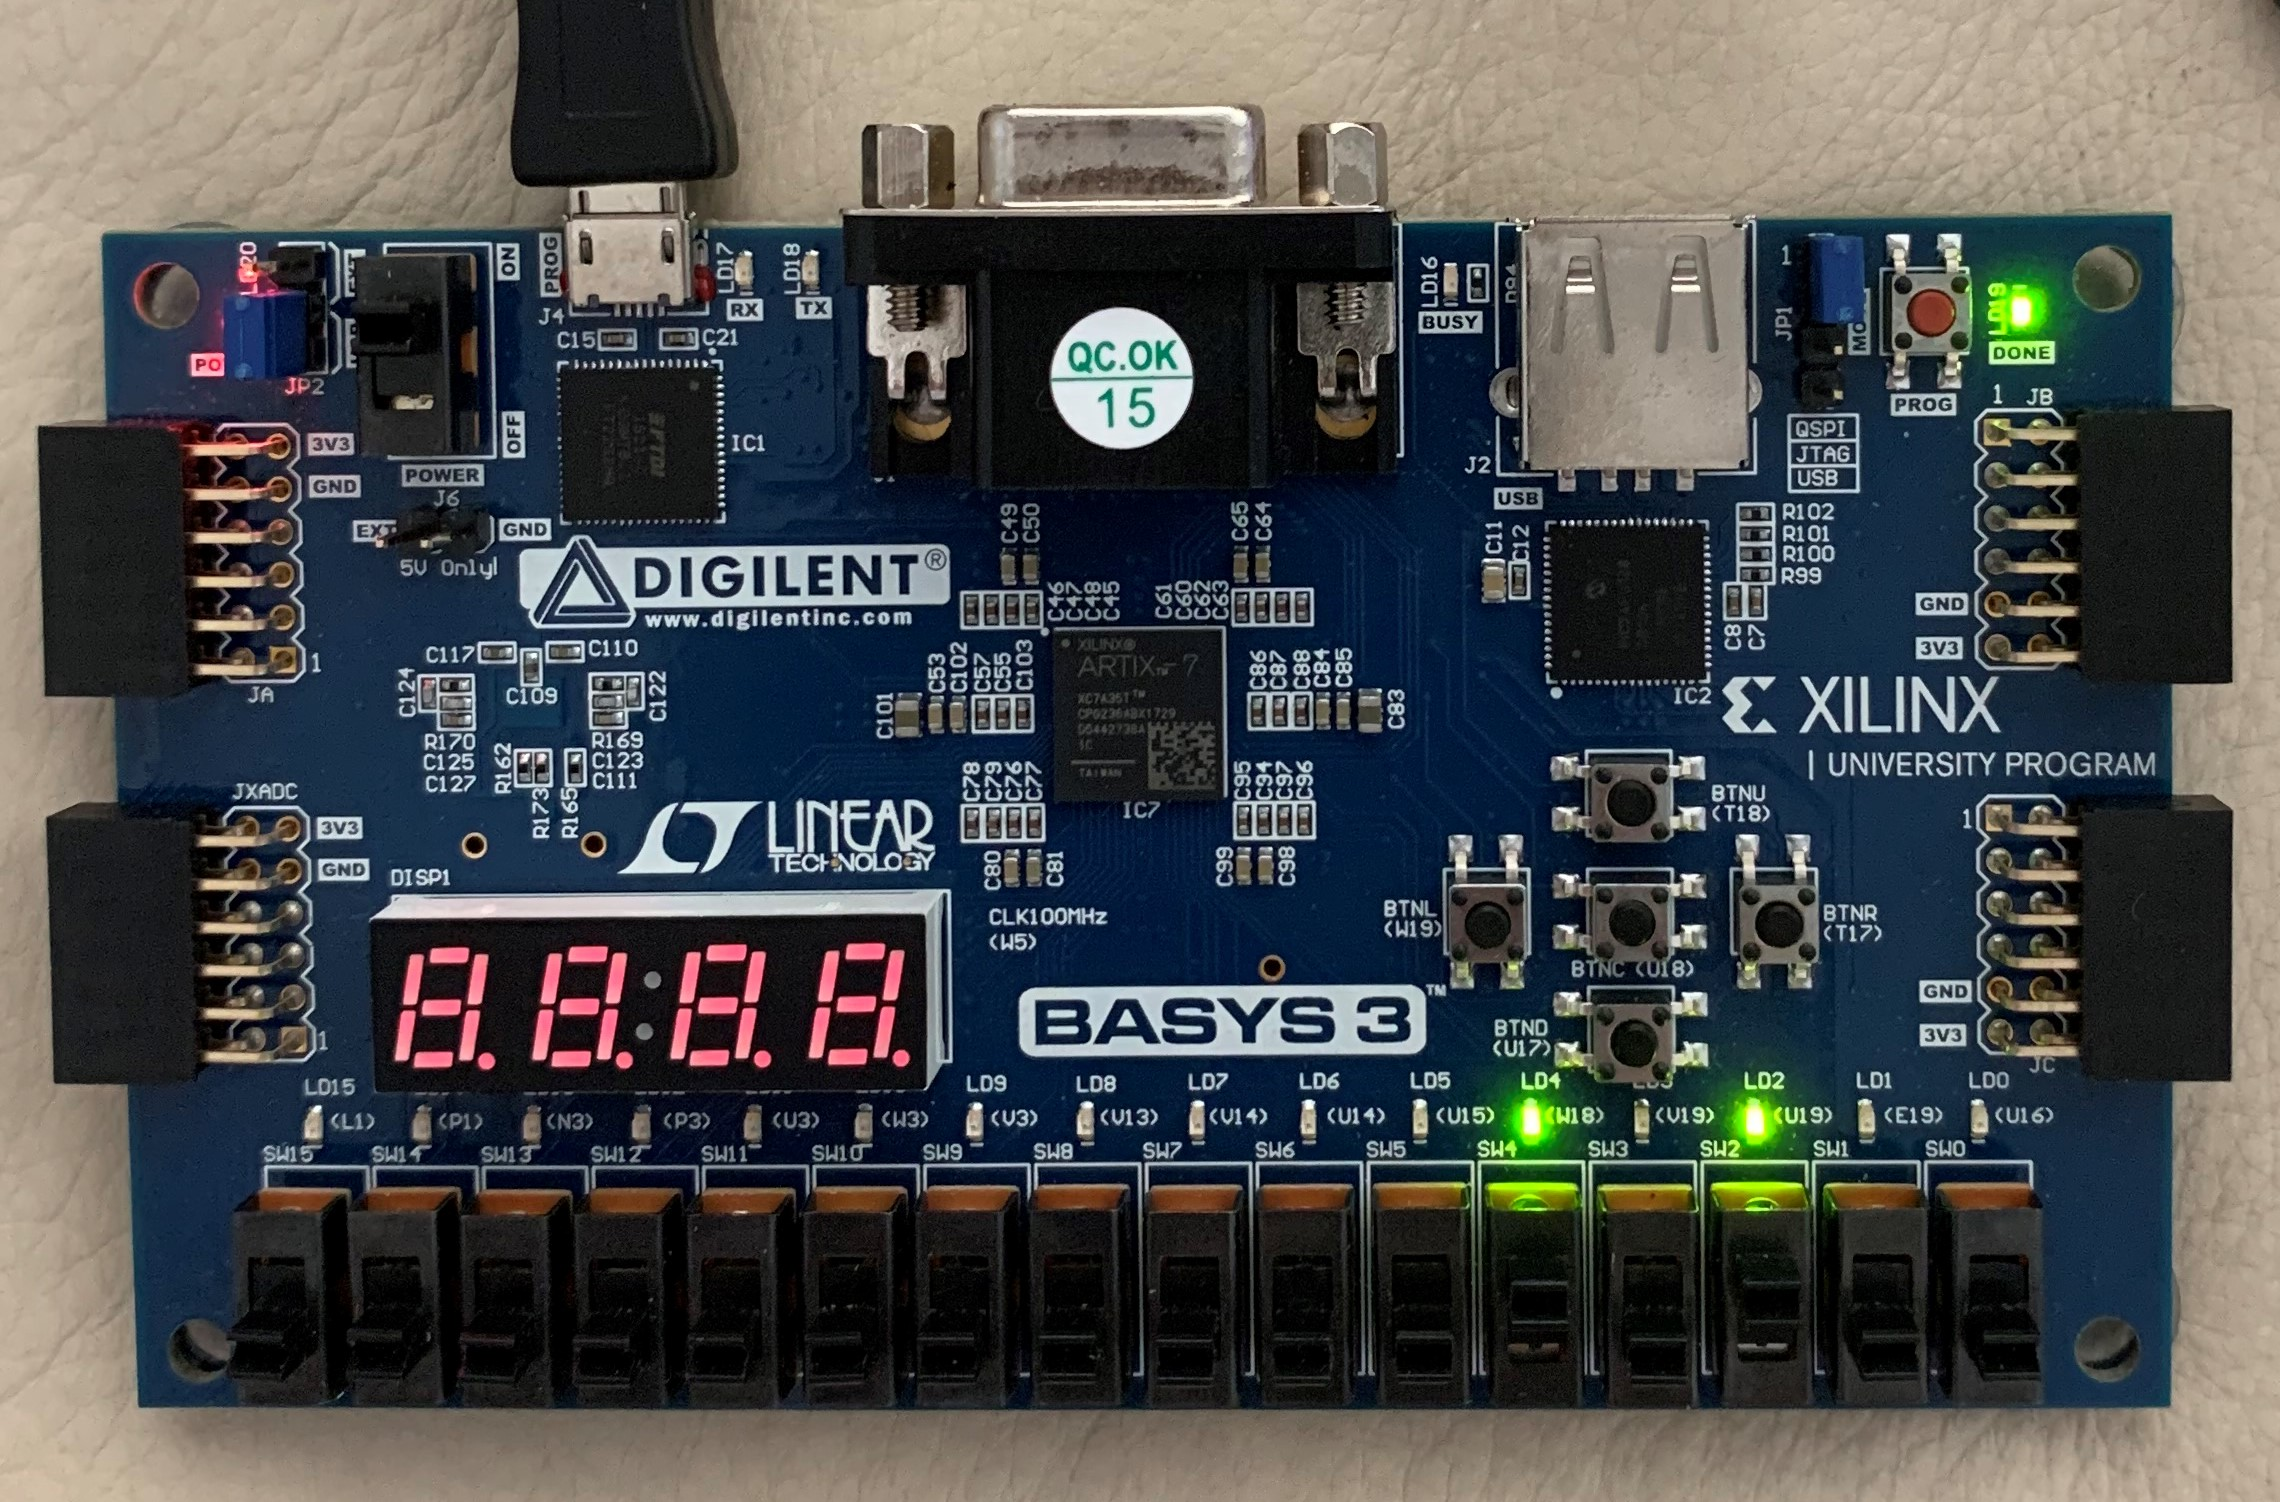
\includegraphics[width=0.8\textwidth,trim=0cm 0cm 0cm 0cm,clip]{add_step_1}
	\caption{Step 1 of ADD (10100)}
	\label{fig:add_step_1}			
\end{figure}

\begin{figure}[ht]\centering
	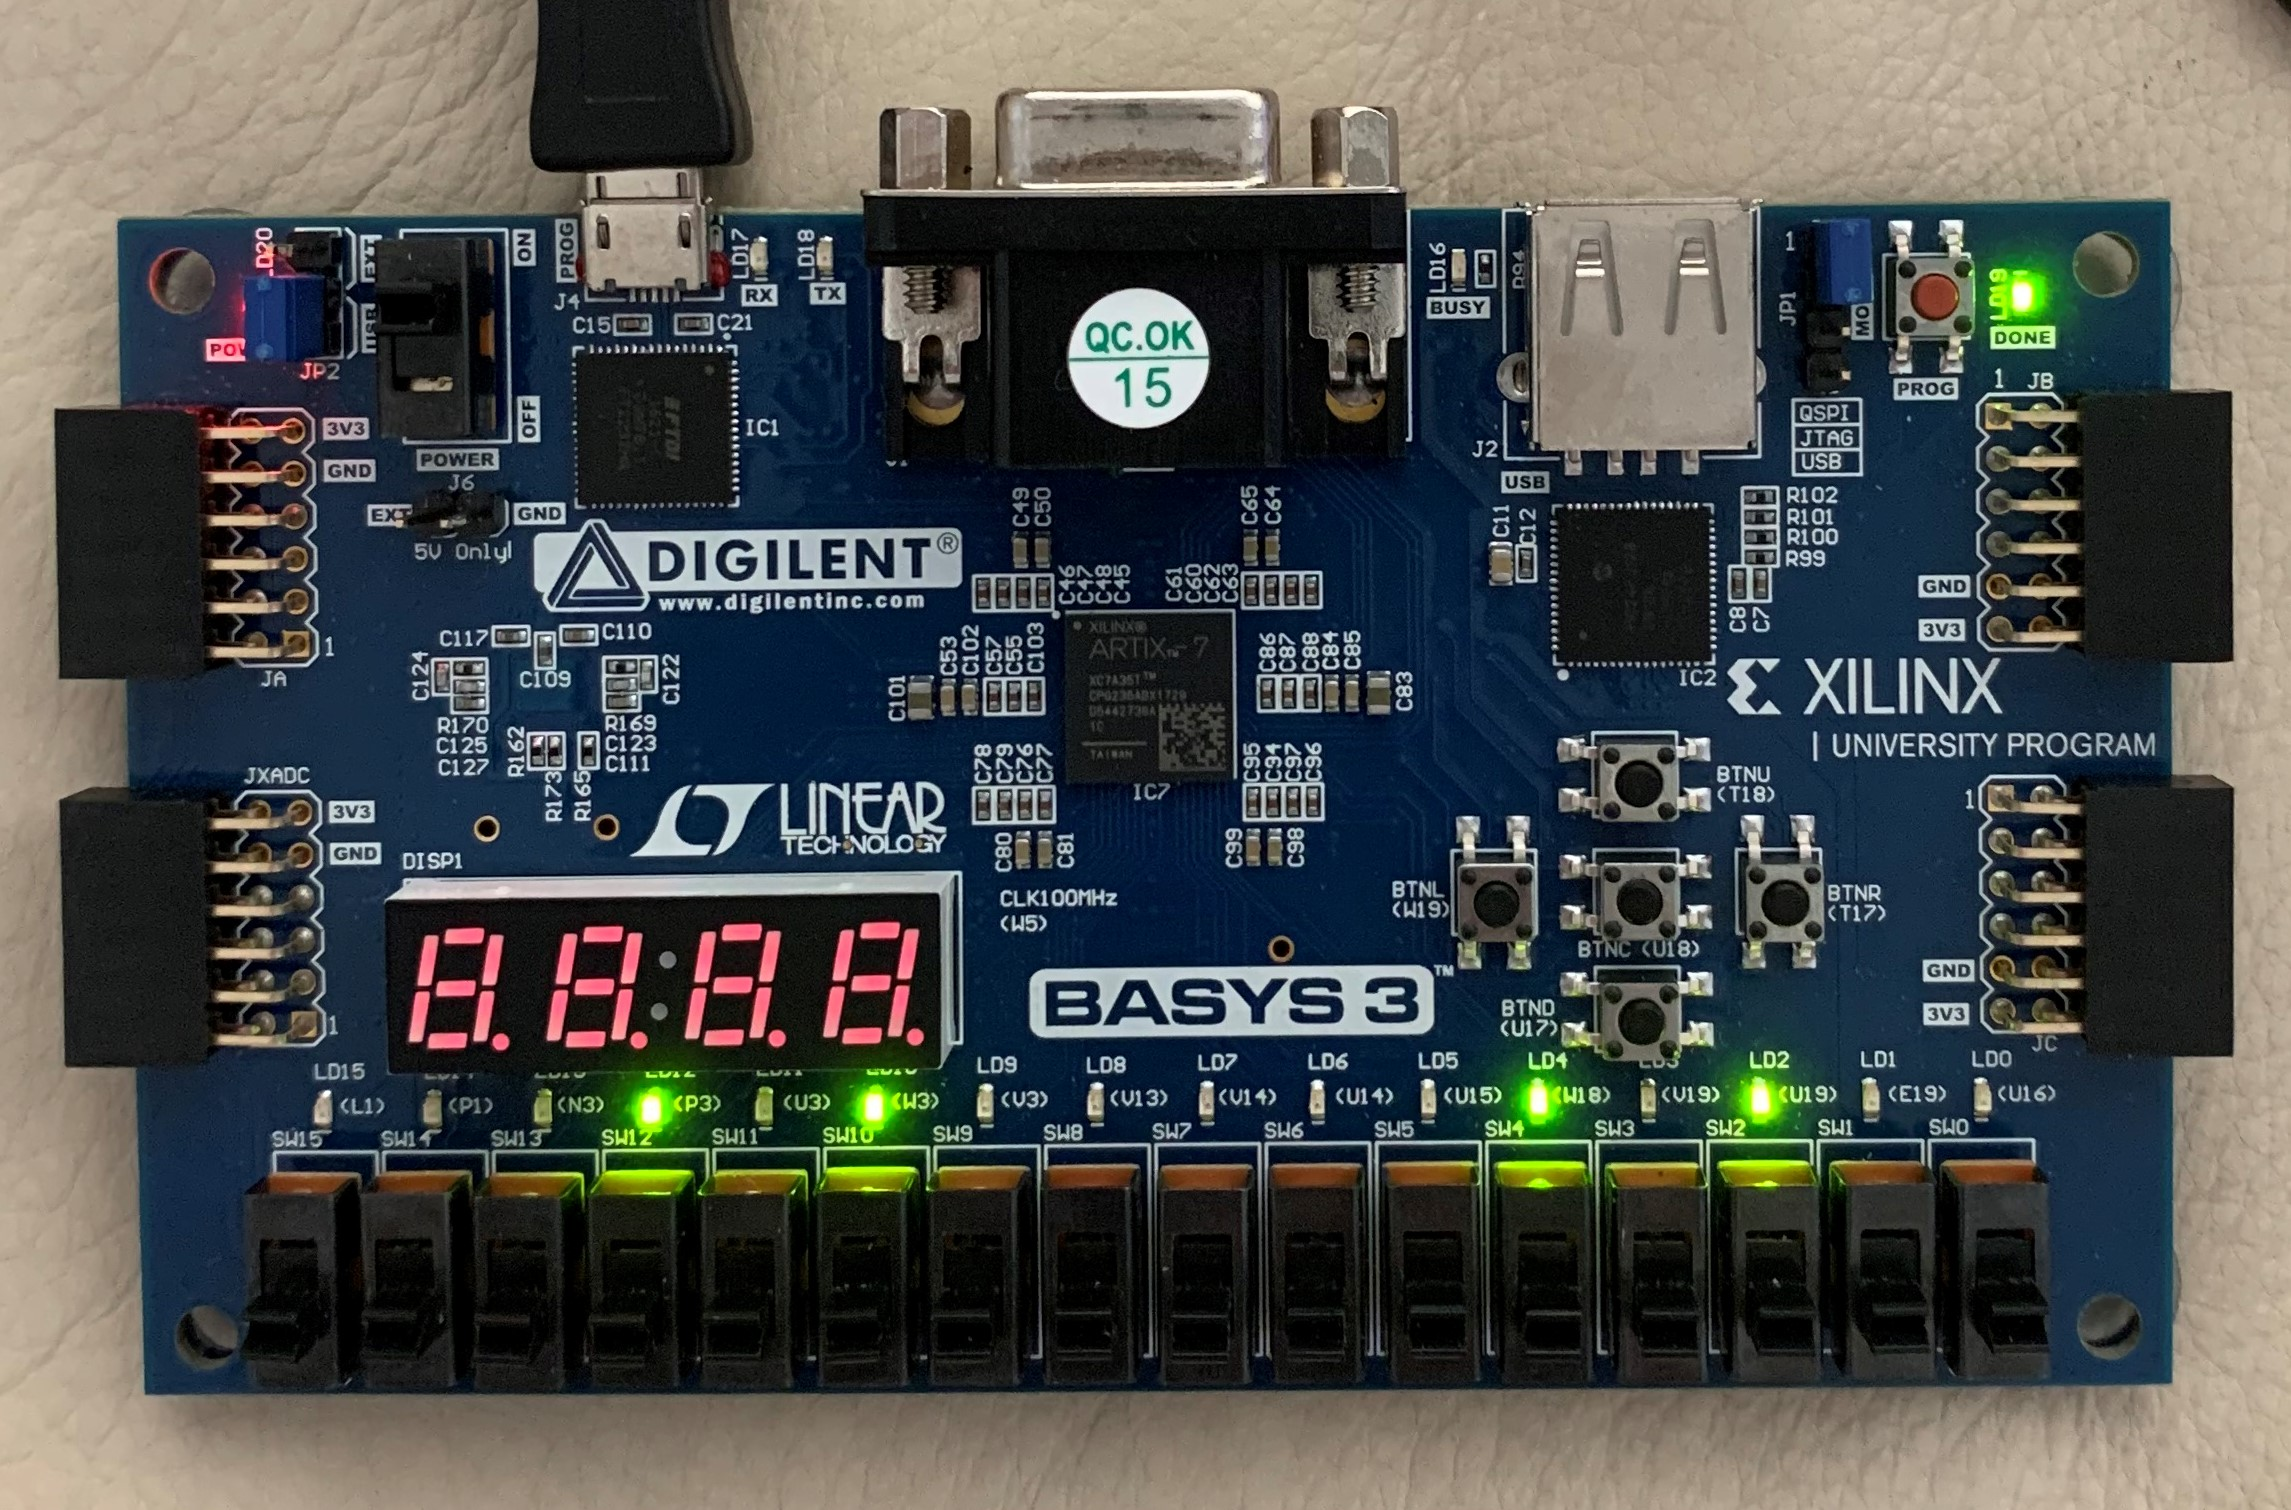
\includegraphics[width=0.8\textwidth,trim=0cm 0cm 0cm 0cm,clip]{add_step_2}
	\caption{Step 2 of ADD (set)}
	\label{fig:add_step_2}			
\end{figure}

\begin{figure}[ht]\centering
	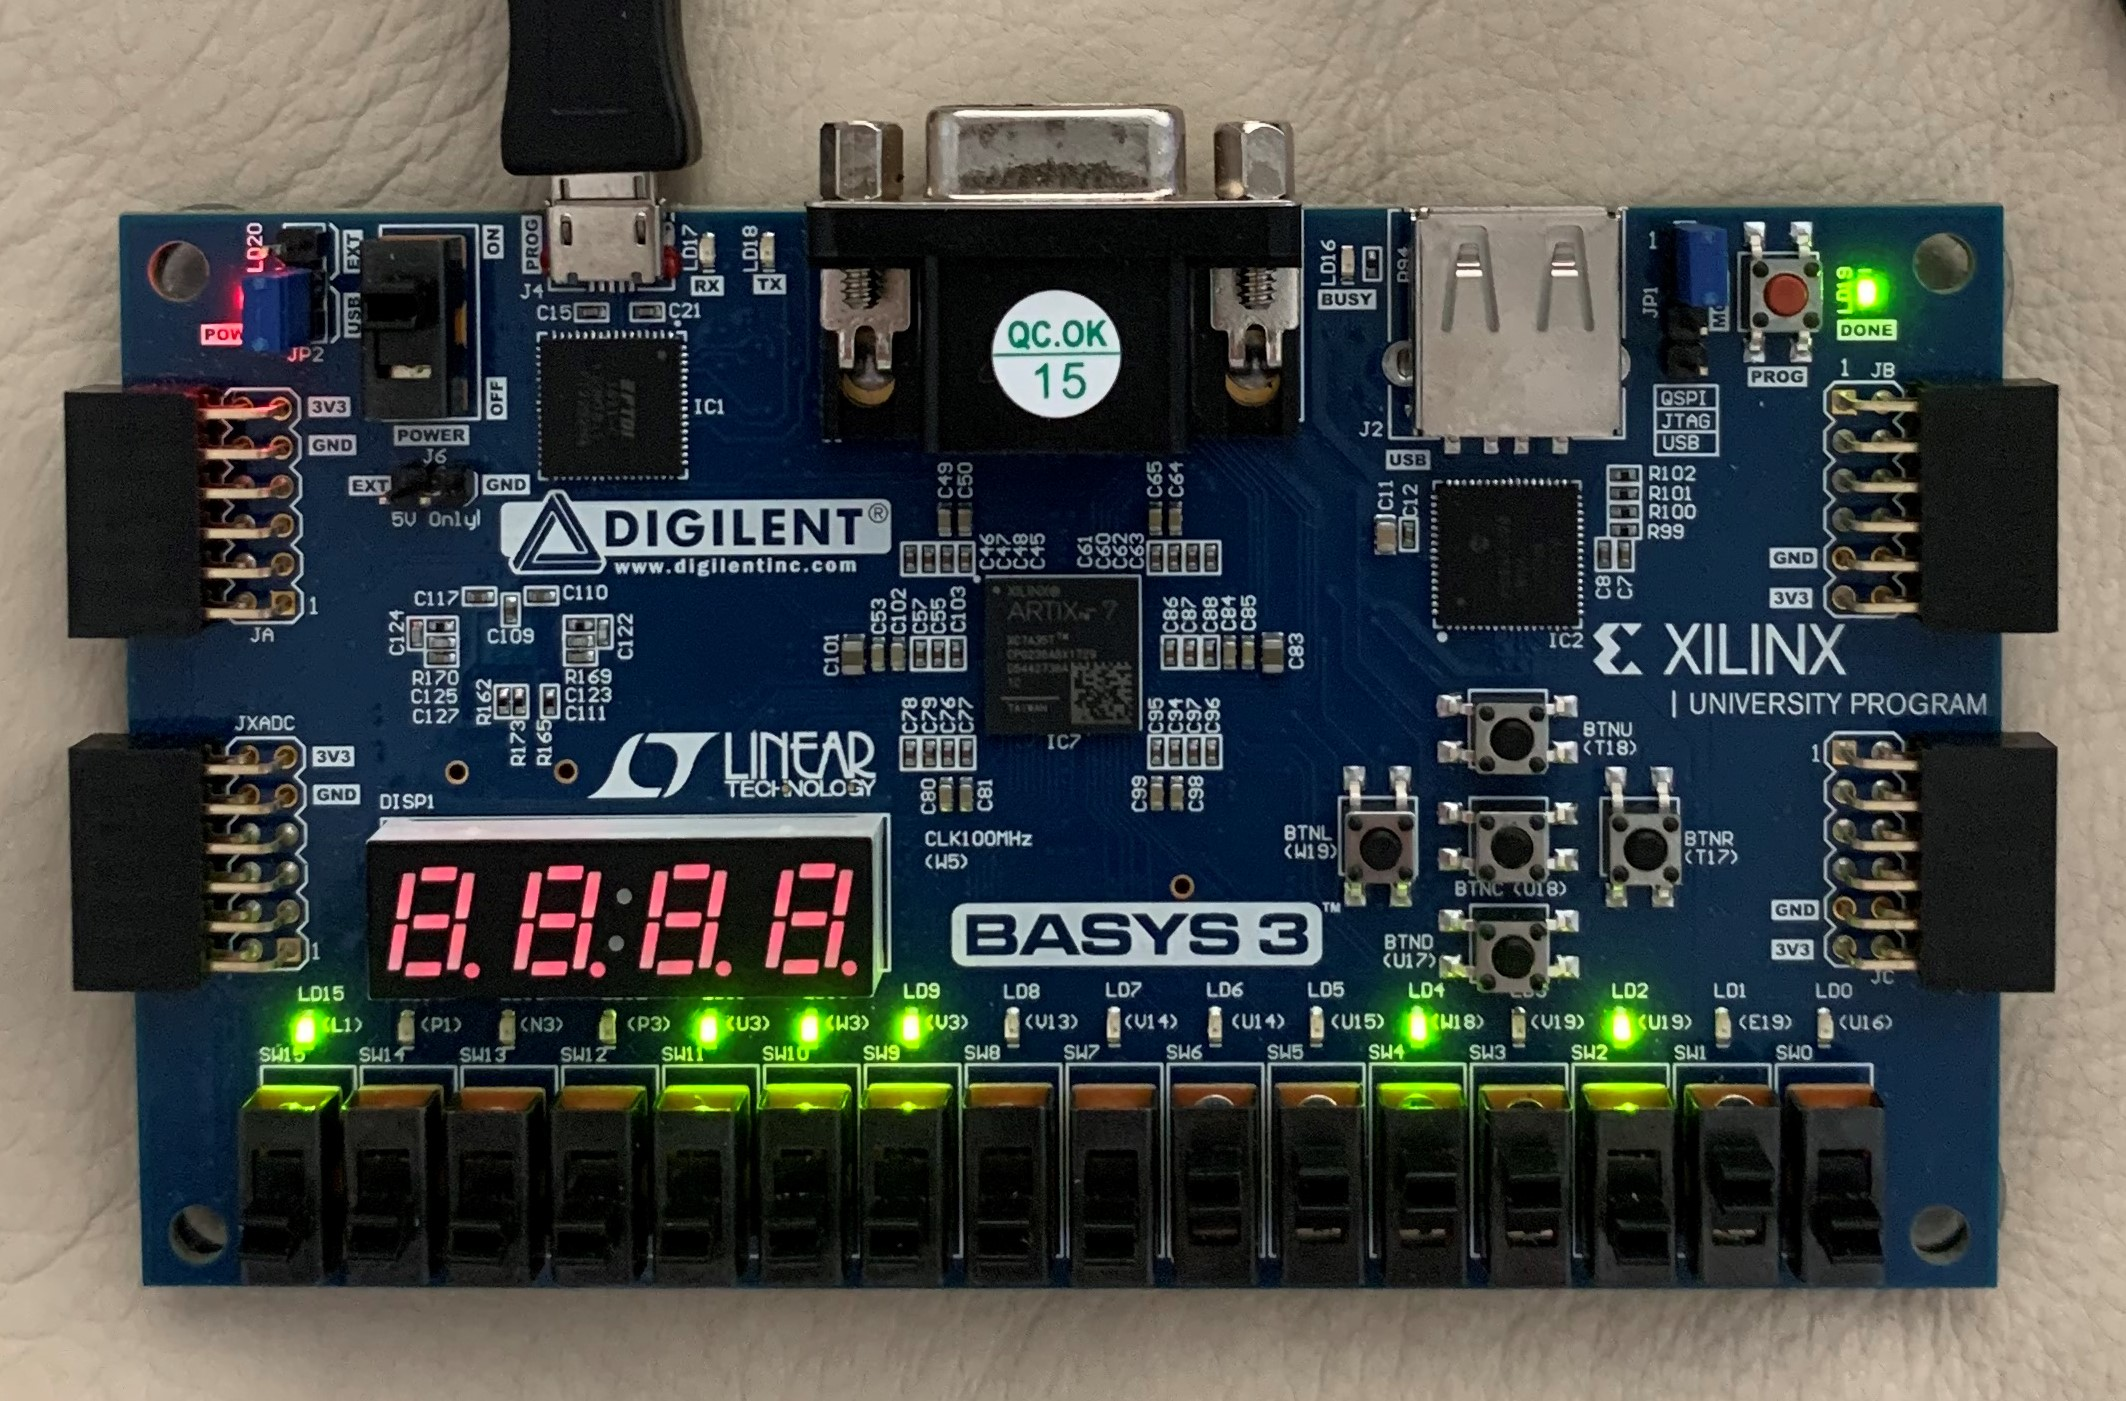
\includegraphics[width=0.8\textwidth,trim=0cm 0cm 0cm 0cm,clip]{add_step_3}
	\caption{Step 3 of ADD (add 111010 to get 10001110)}
	\label{fig:add_step_3}			
\end{figure}
\clearpage

\section*{Op 1: SUB}

\begin{figure}[ht]\centering
	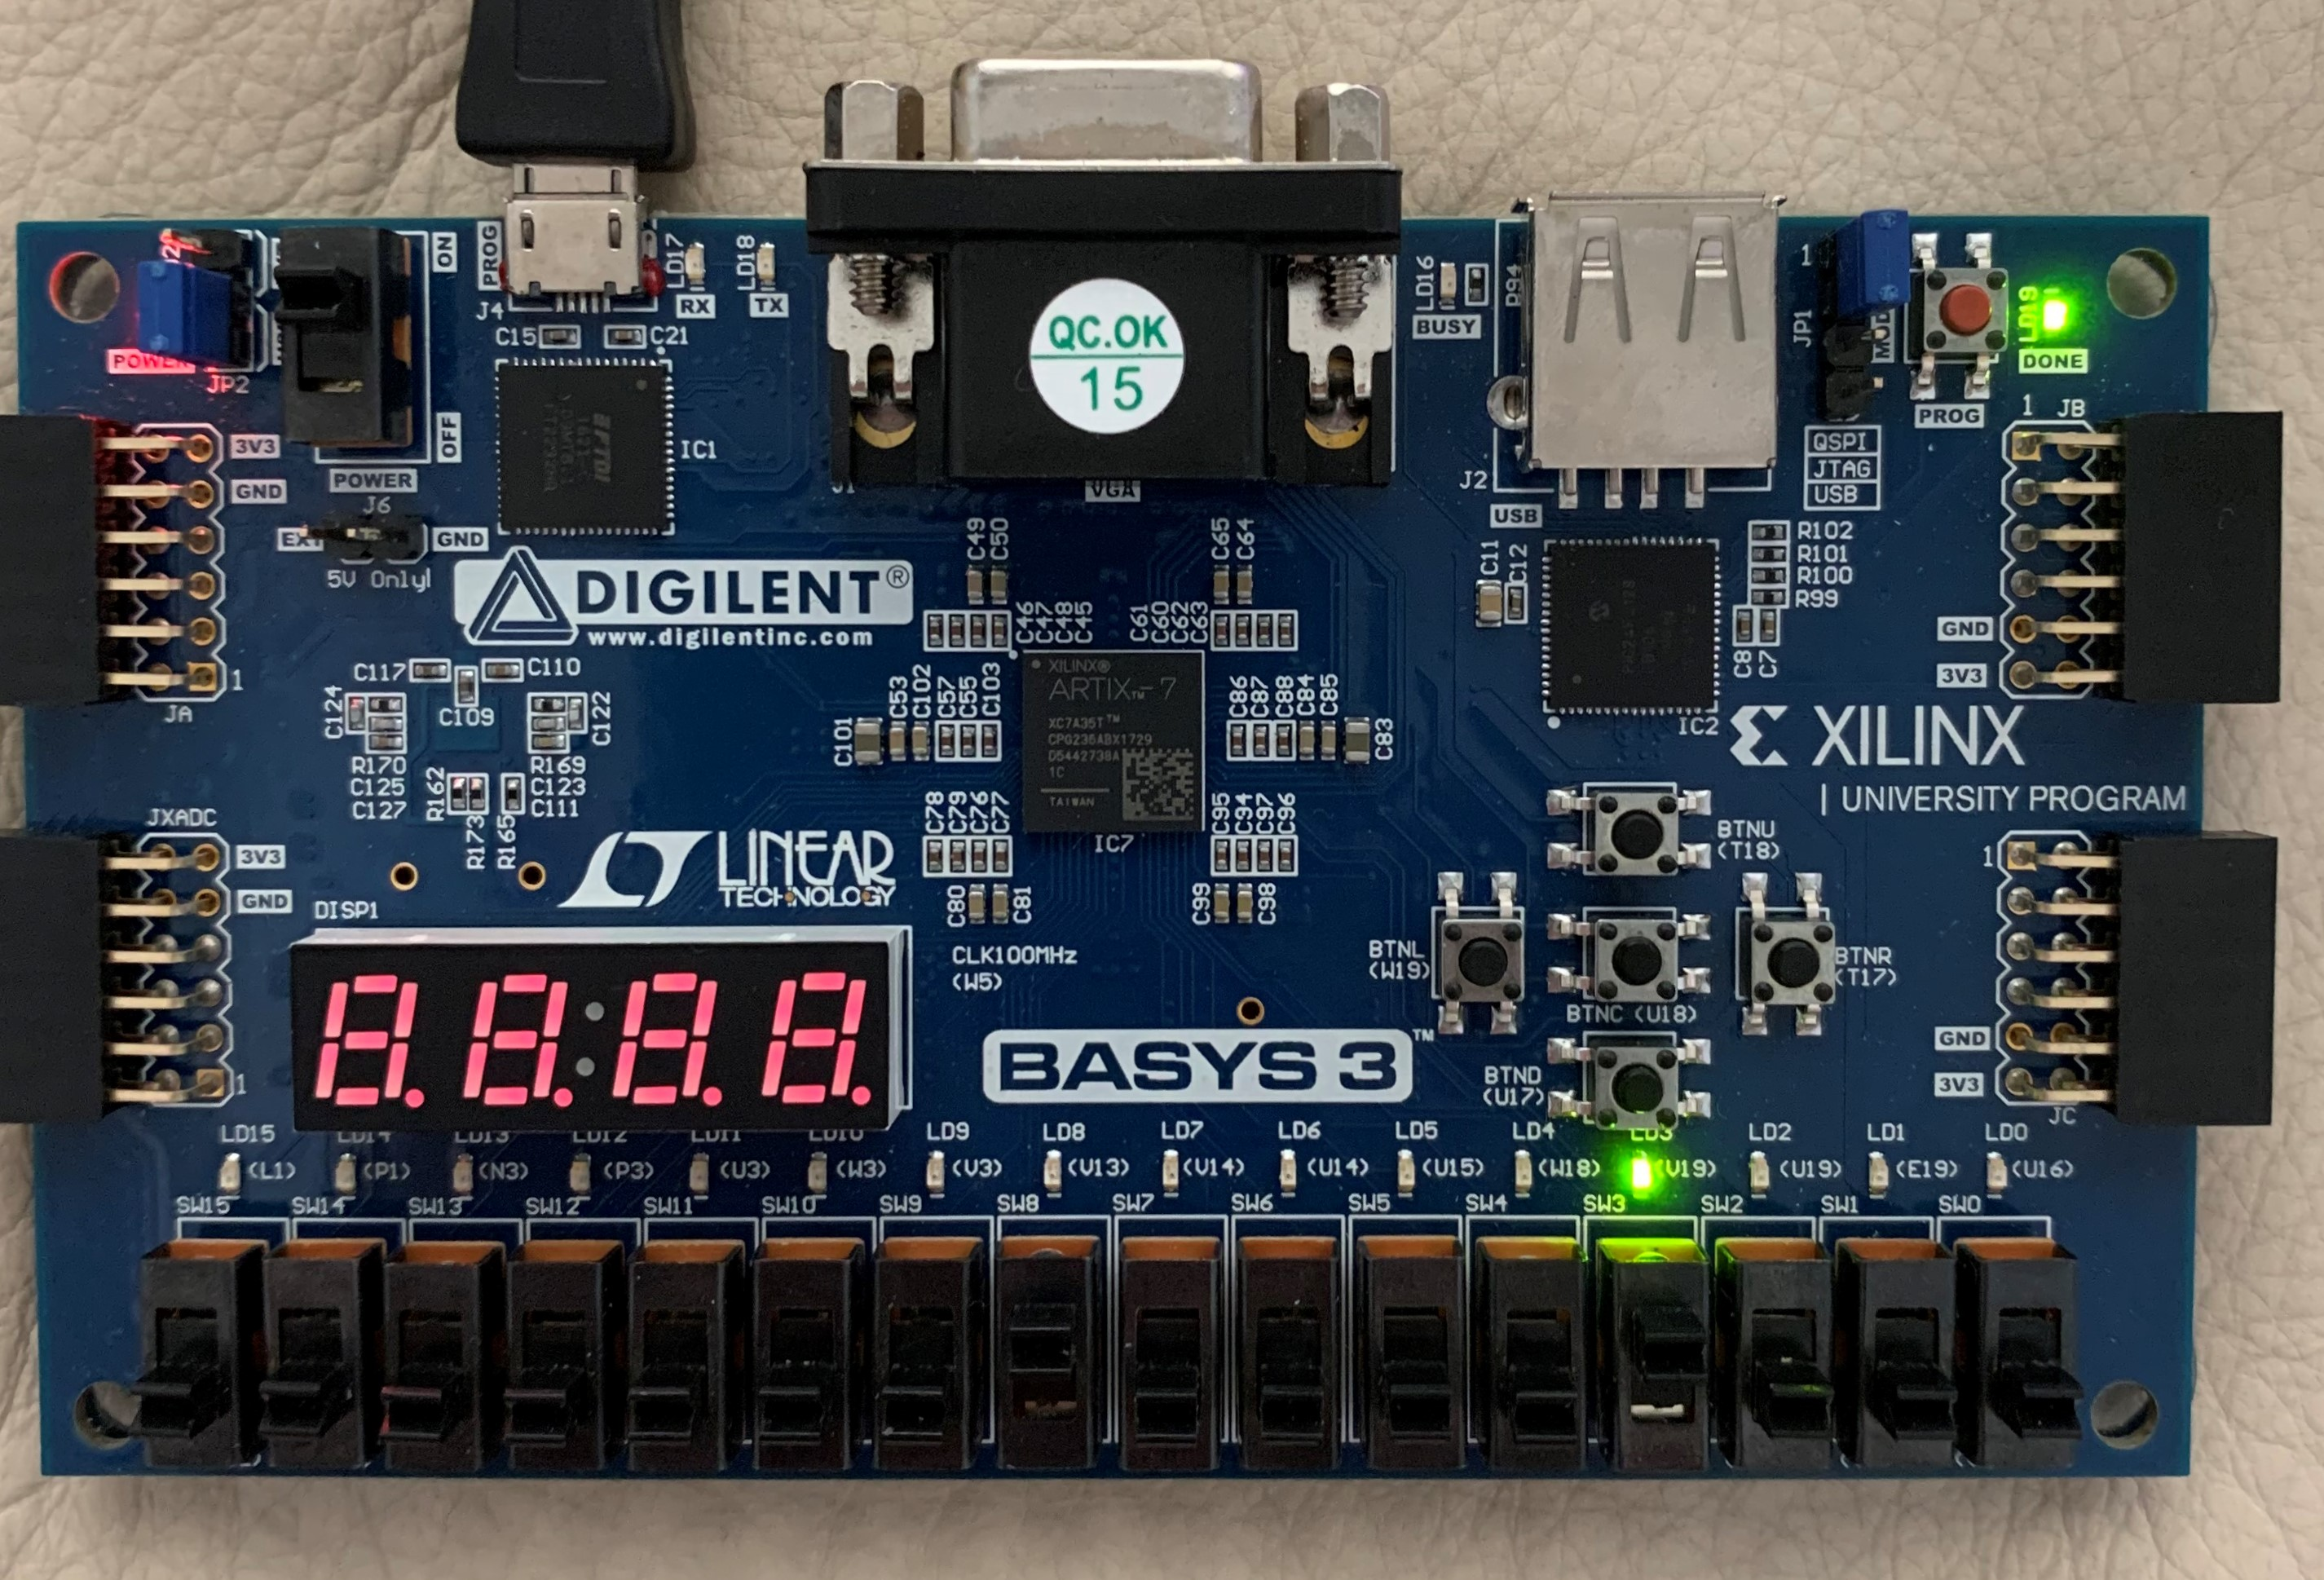
\includegraphics[width=0.8\textwidth,trim=0cm 0cm 0cm 0cm,clip]{sub_step_1}
	\caption{Step 1 of SUB (start with 1000)}
	\label{fig:sub_step_1}			
\end{figure}

\begin{figure}[ht]\centering
	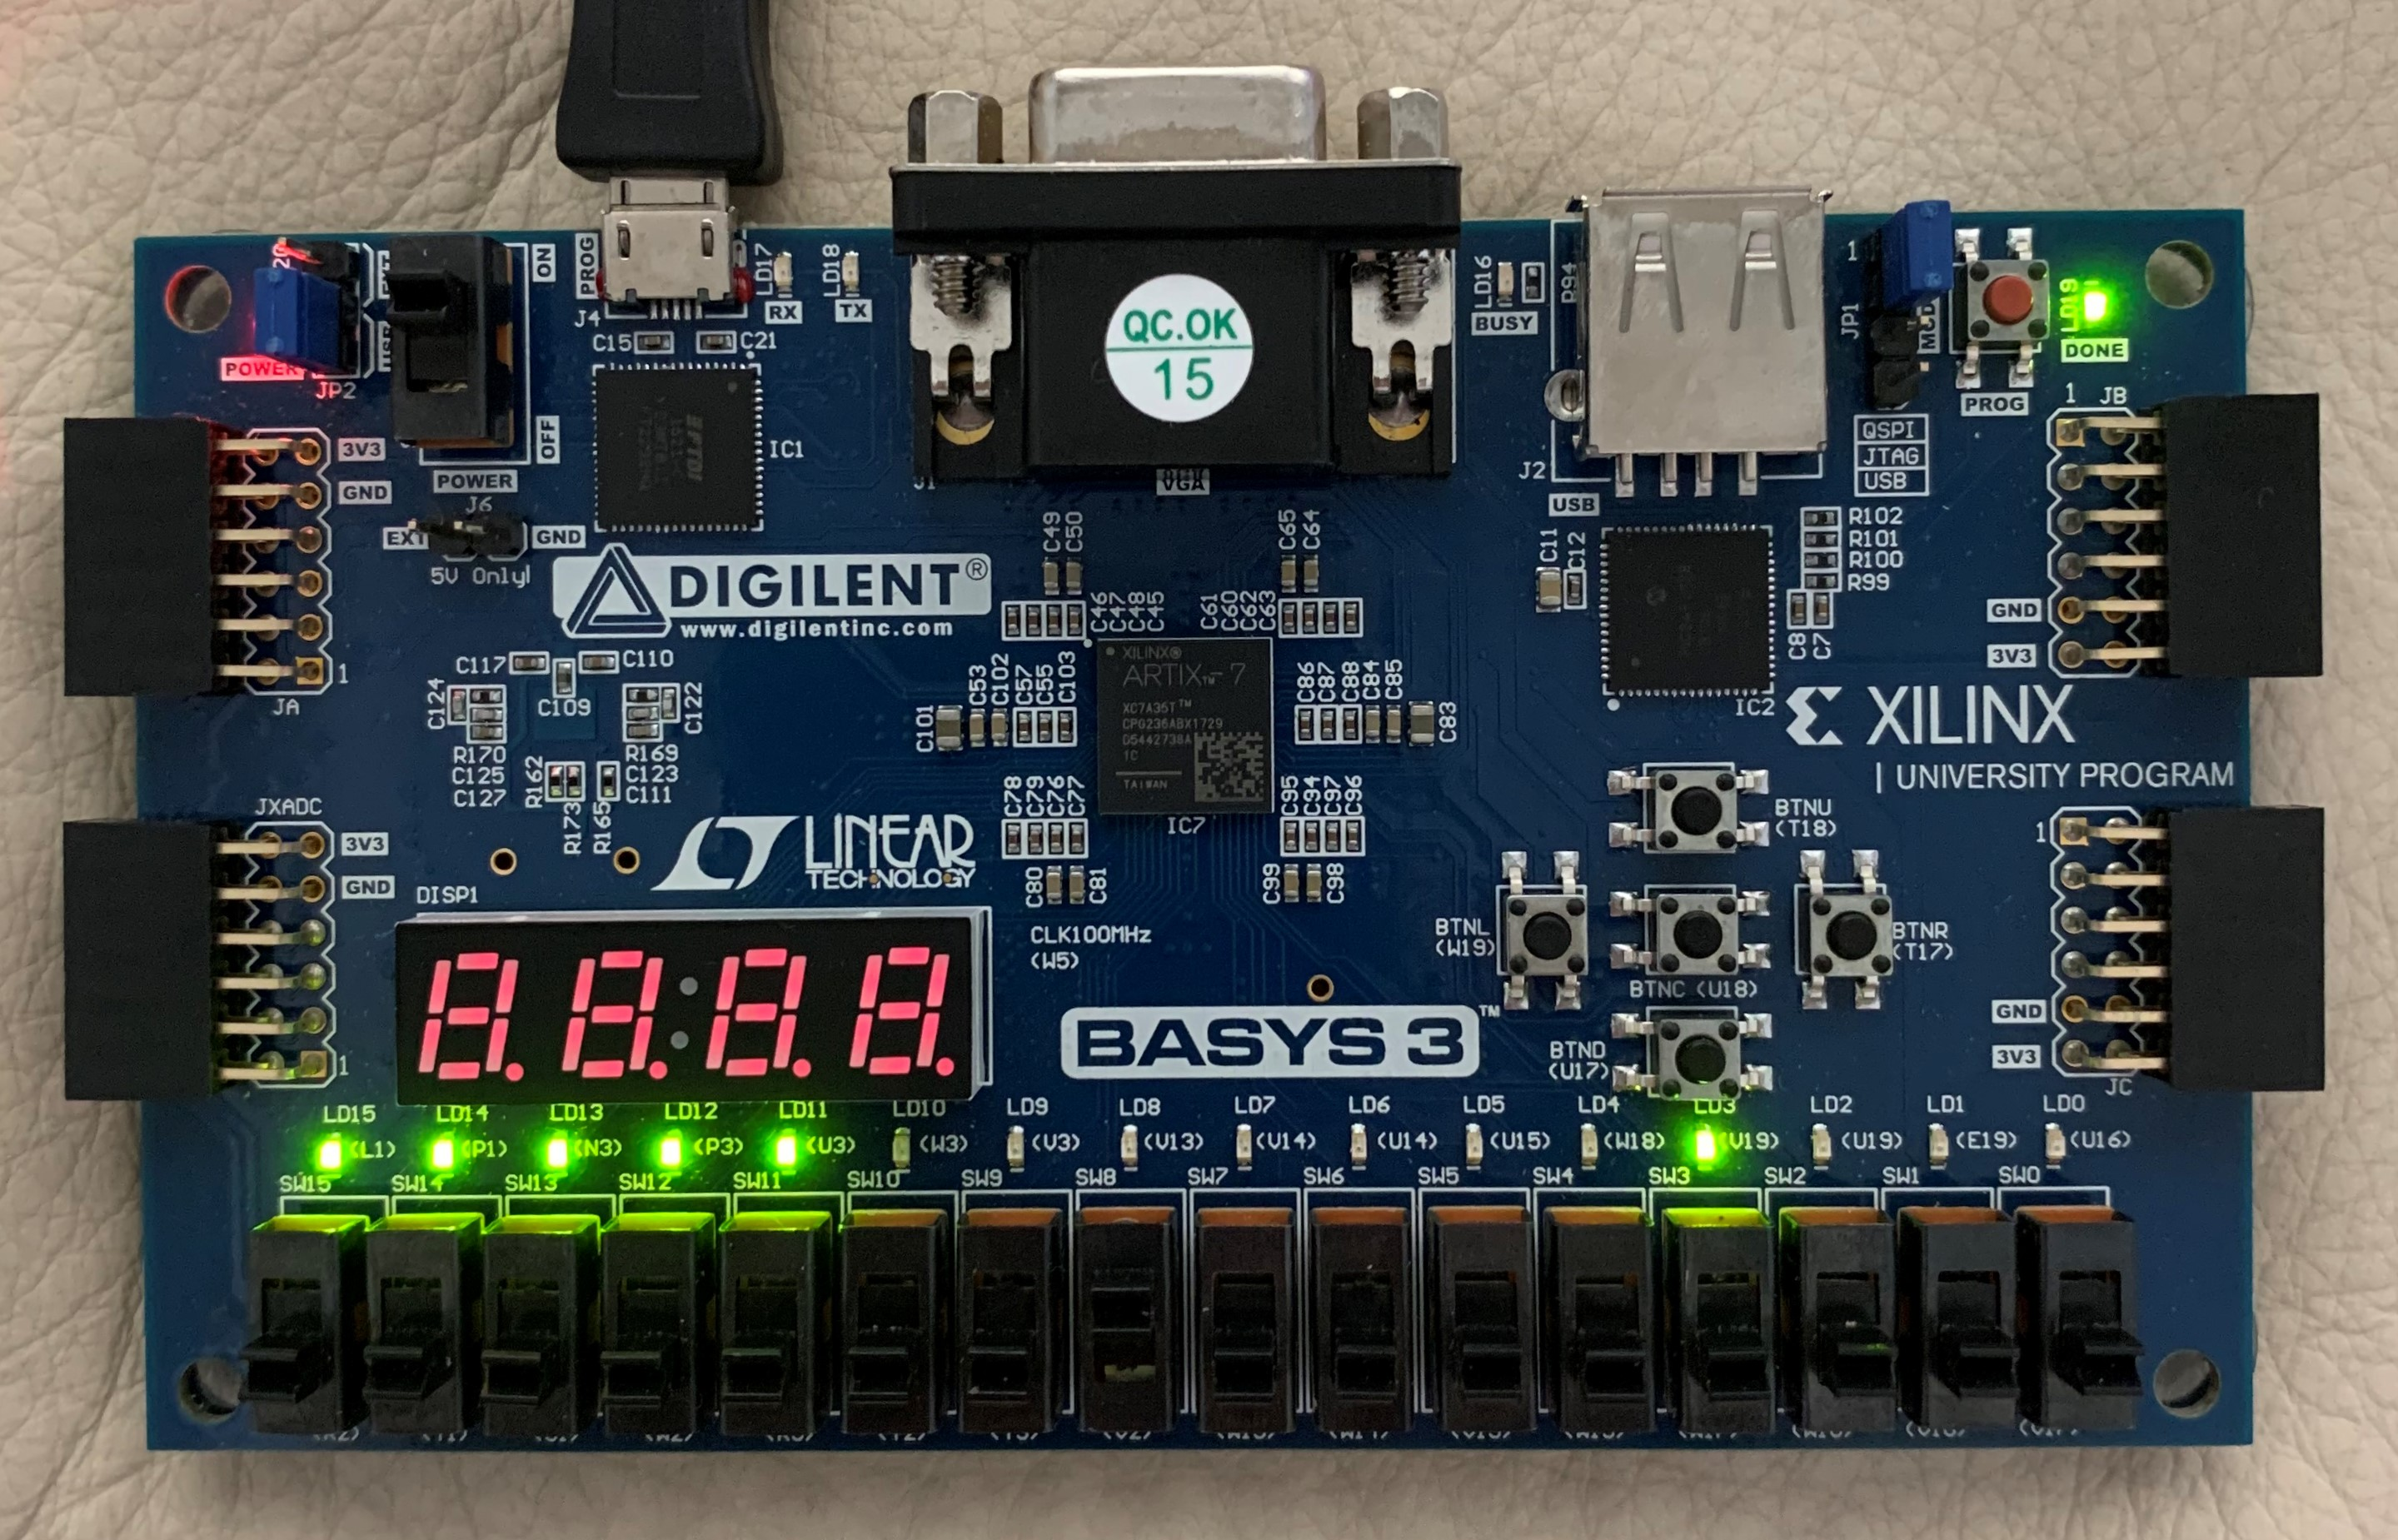
\includegraphics[width=0.8\textwidth,trim=0cm 0cm 0cm 0cm,clip]{sub_step_2}
	\caption{Step 2 of SUB (set)}
	\label{fig:sub_step_2}			
\end{figure}

\begin{figure}[ht]\centering
	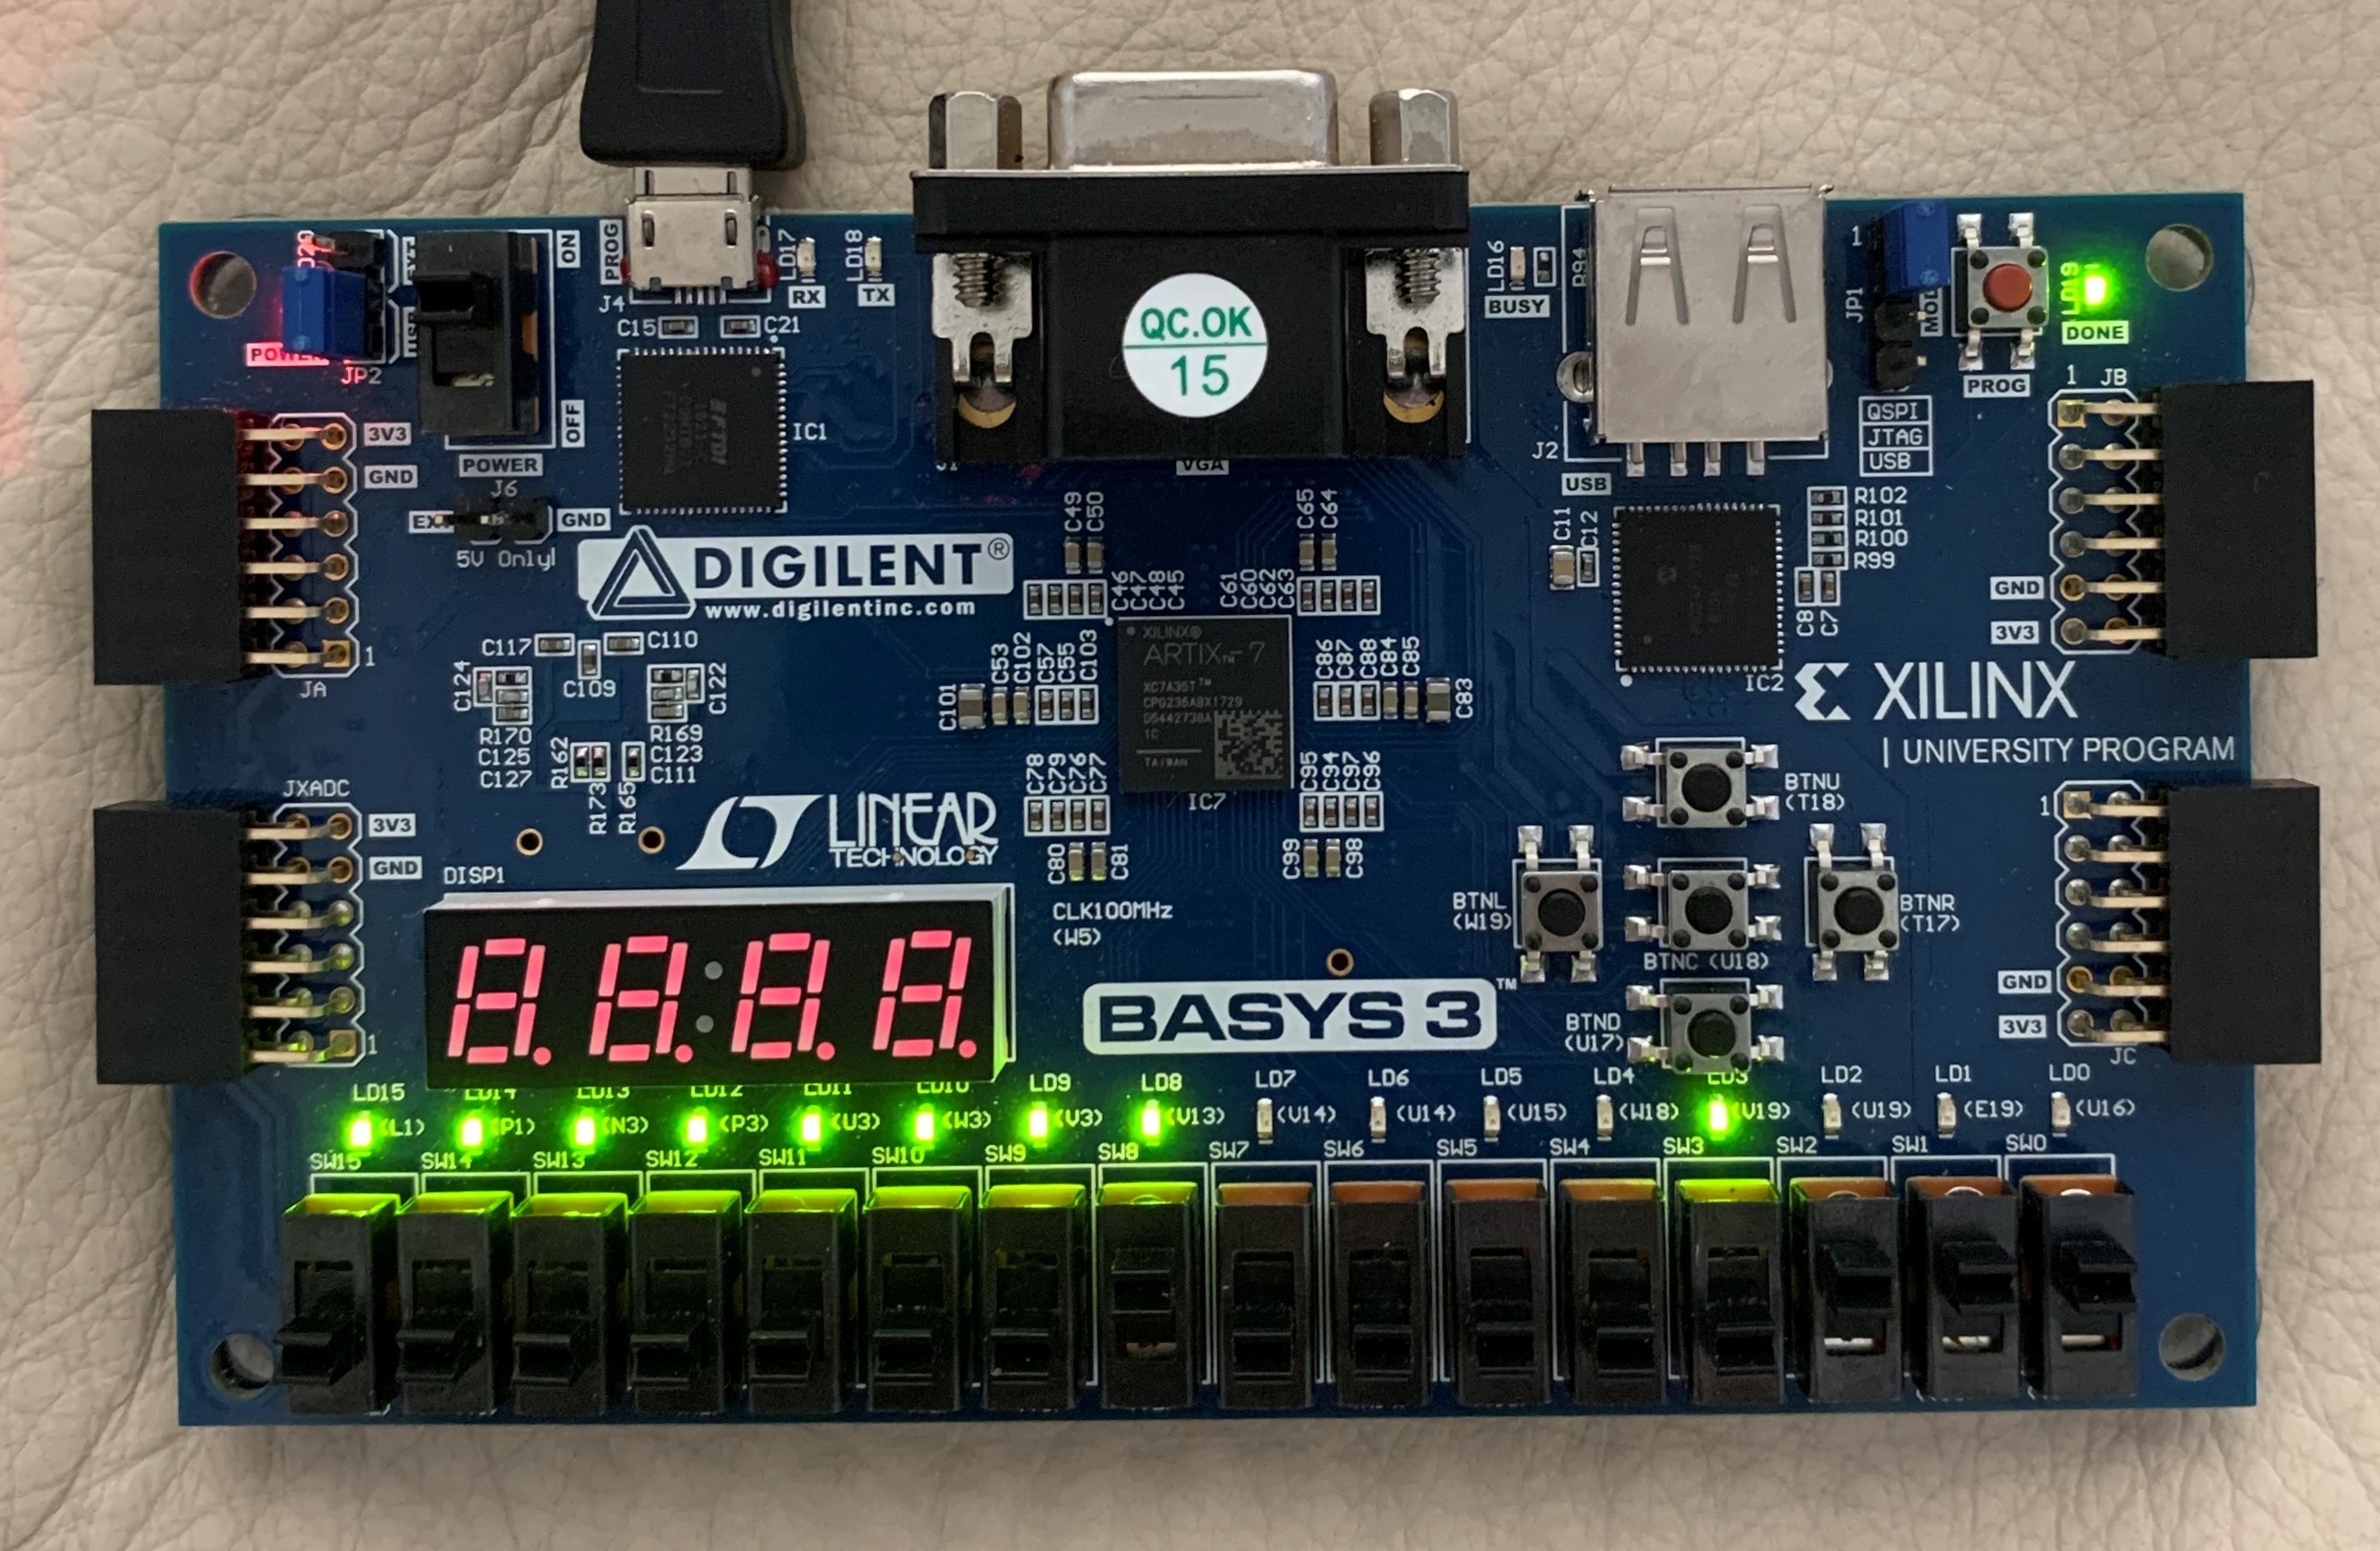
\includegraphics[width=0.8\textwidth,trim=0cm 0cm 0cm 0cm,clip]{sub_step_3}
	\caption{Step 3 of SUB (subtract 111)}
	\label{fig:sub_step_3}			
\end{figure}
\clearpage

\section*{Op 2: AND}

\begin{figure}[ht]\centering
	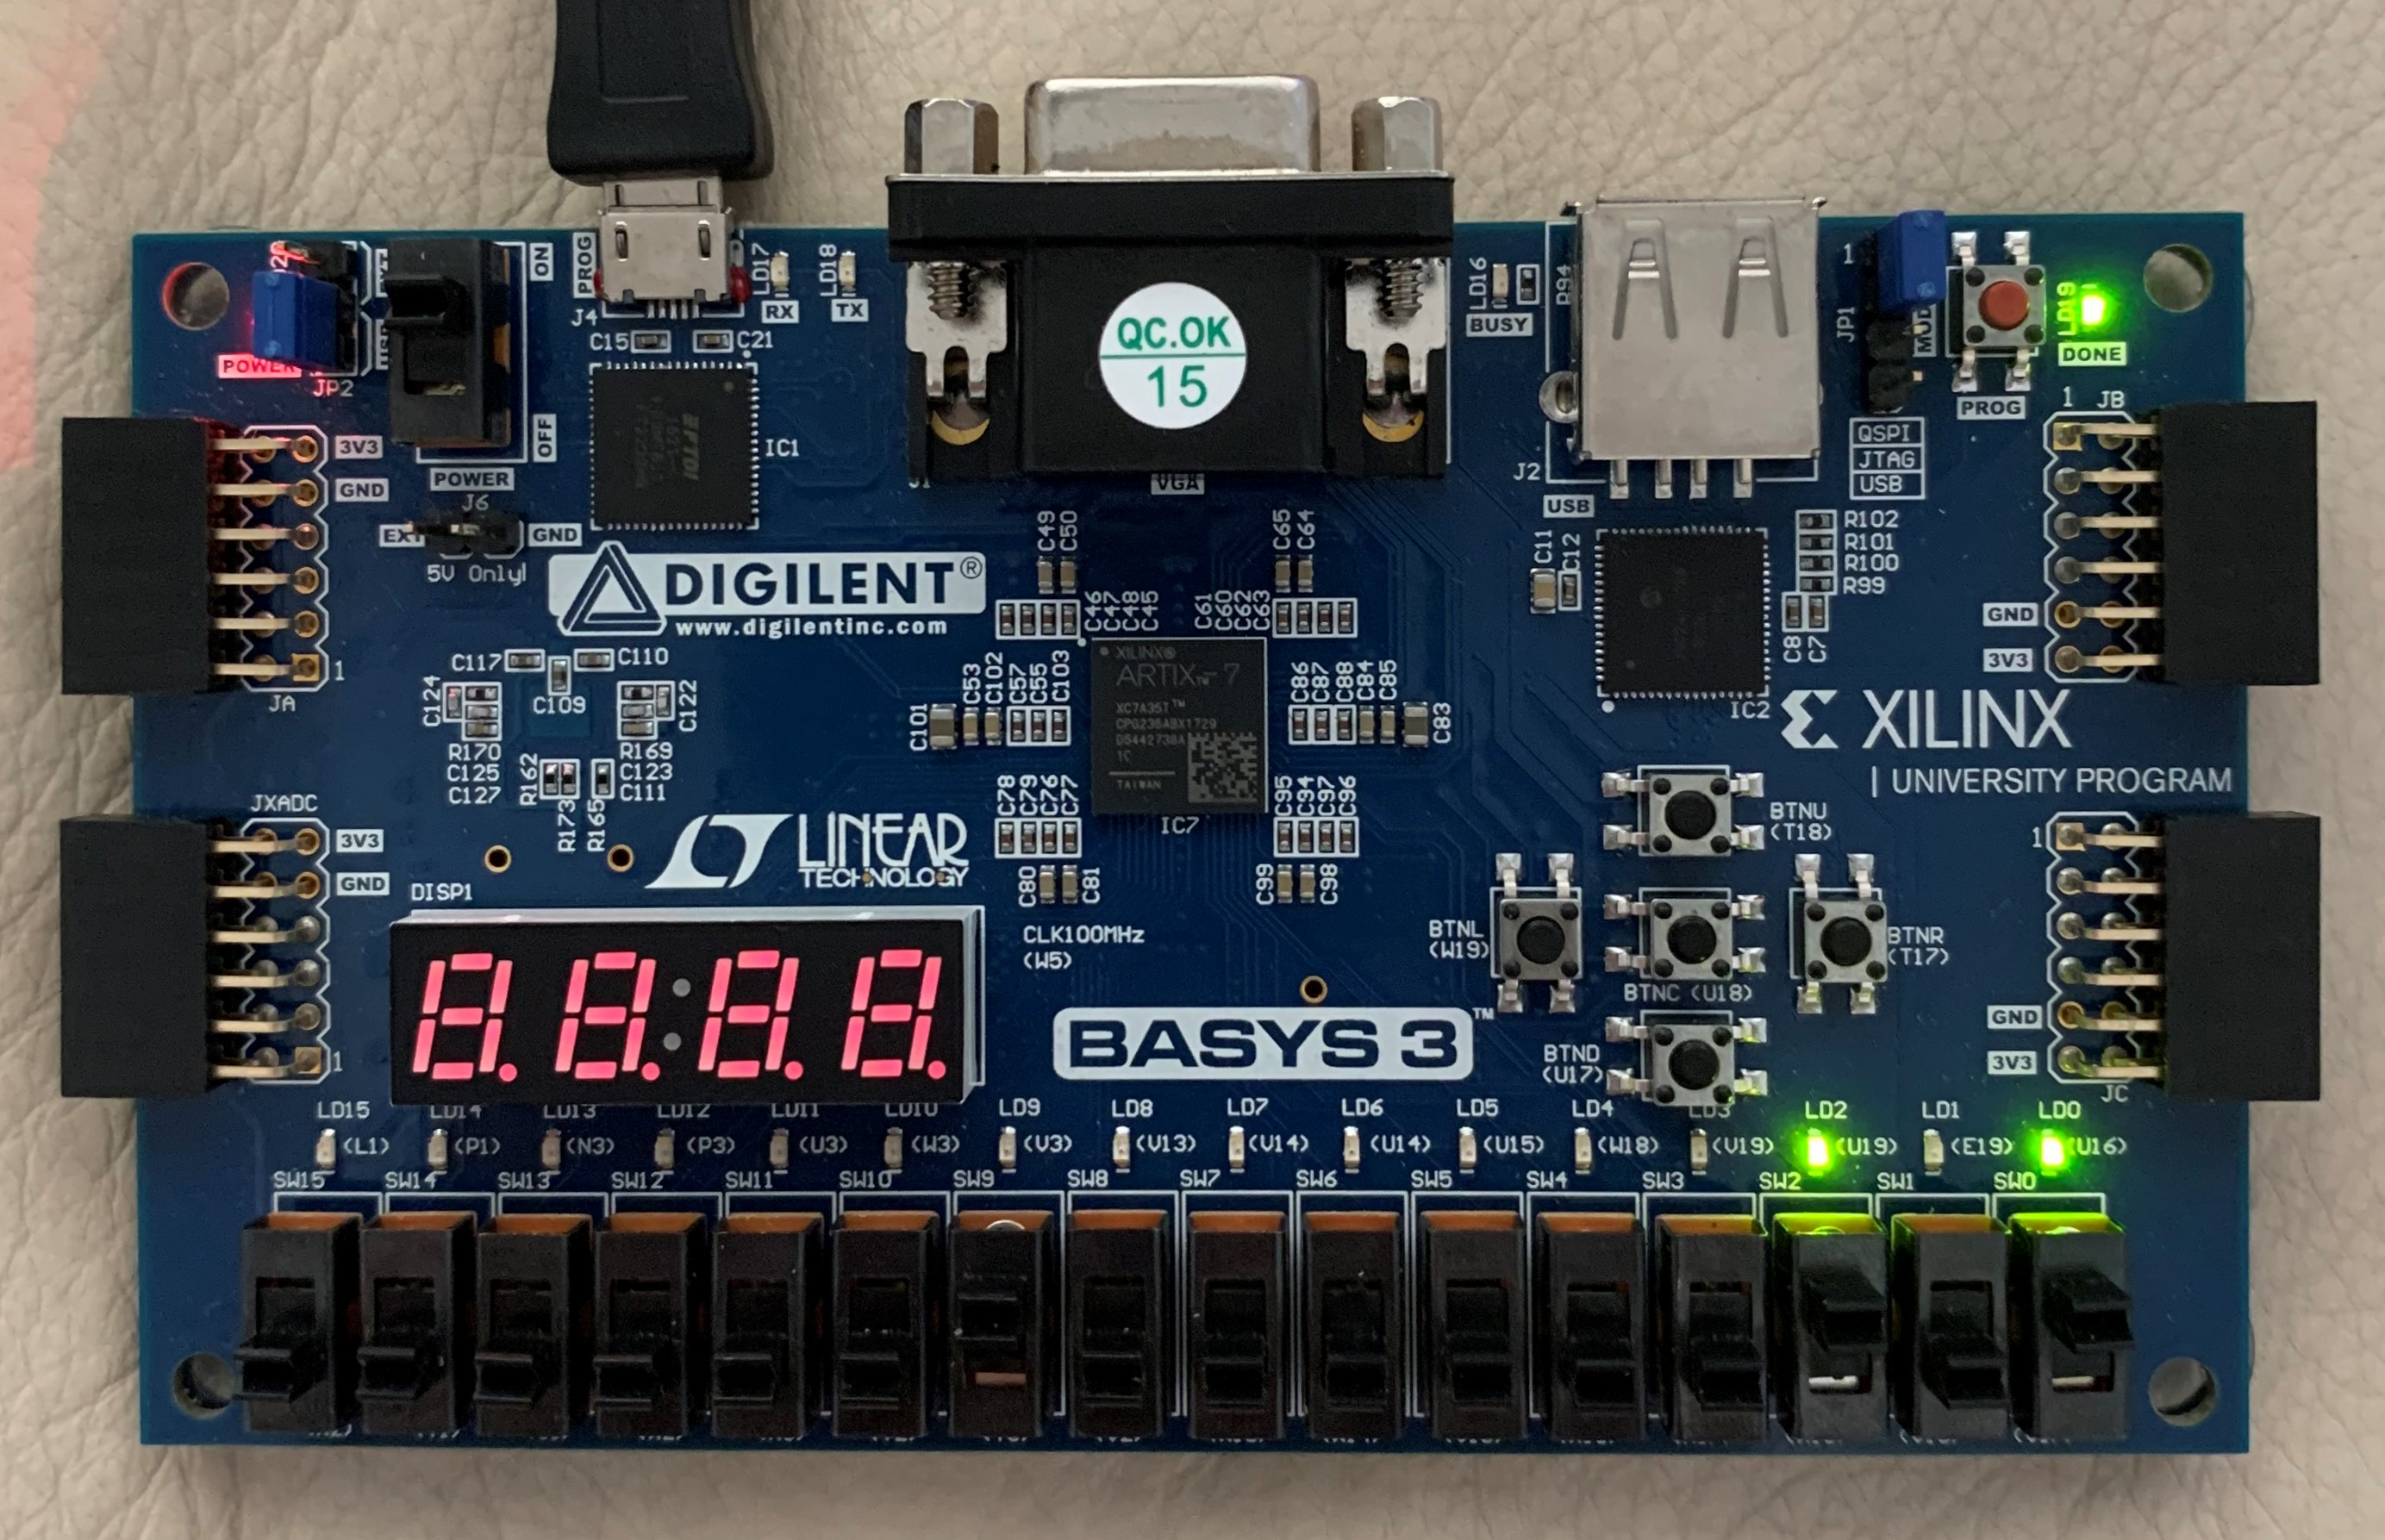
\includegraphics[width=0.8\textwidth,trim=0cm 0cm 0cm 0cm,clip]{and_step_1}
	\caption{Step 1 of AND (start with 101)}
	\label{fig:and_step_1}			
\end{figure}

\begin{figure}[ht]\centering
	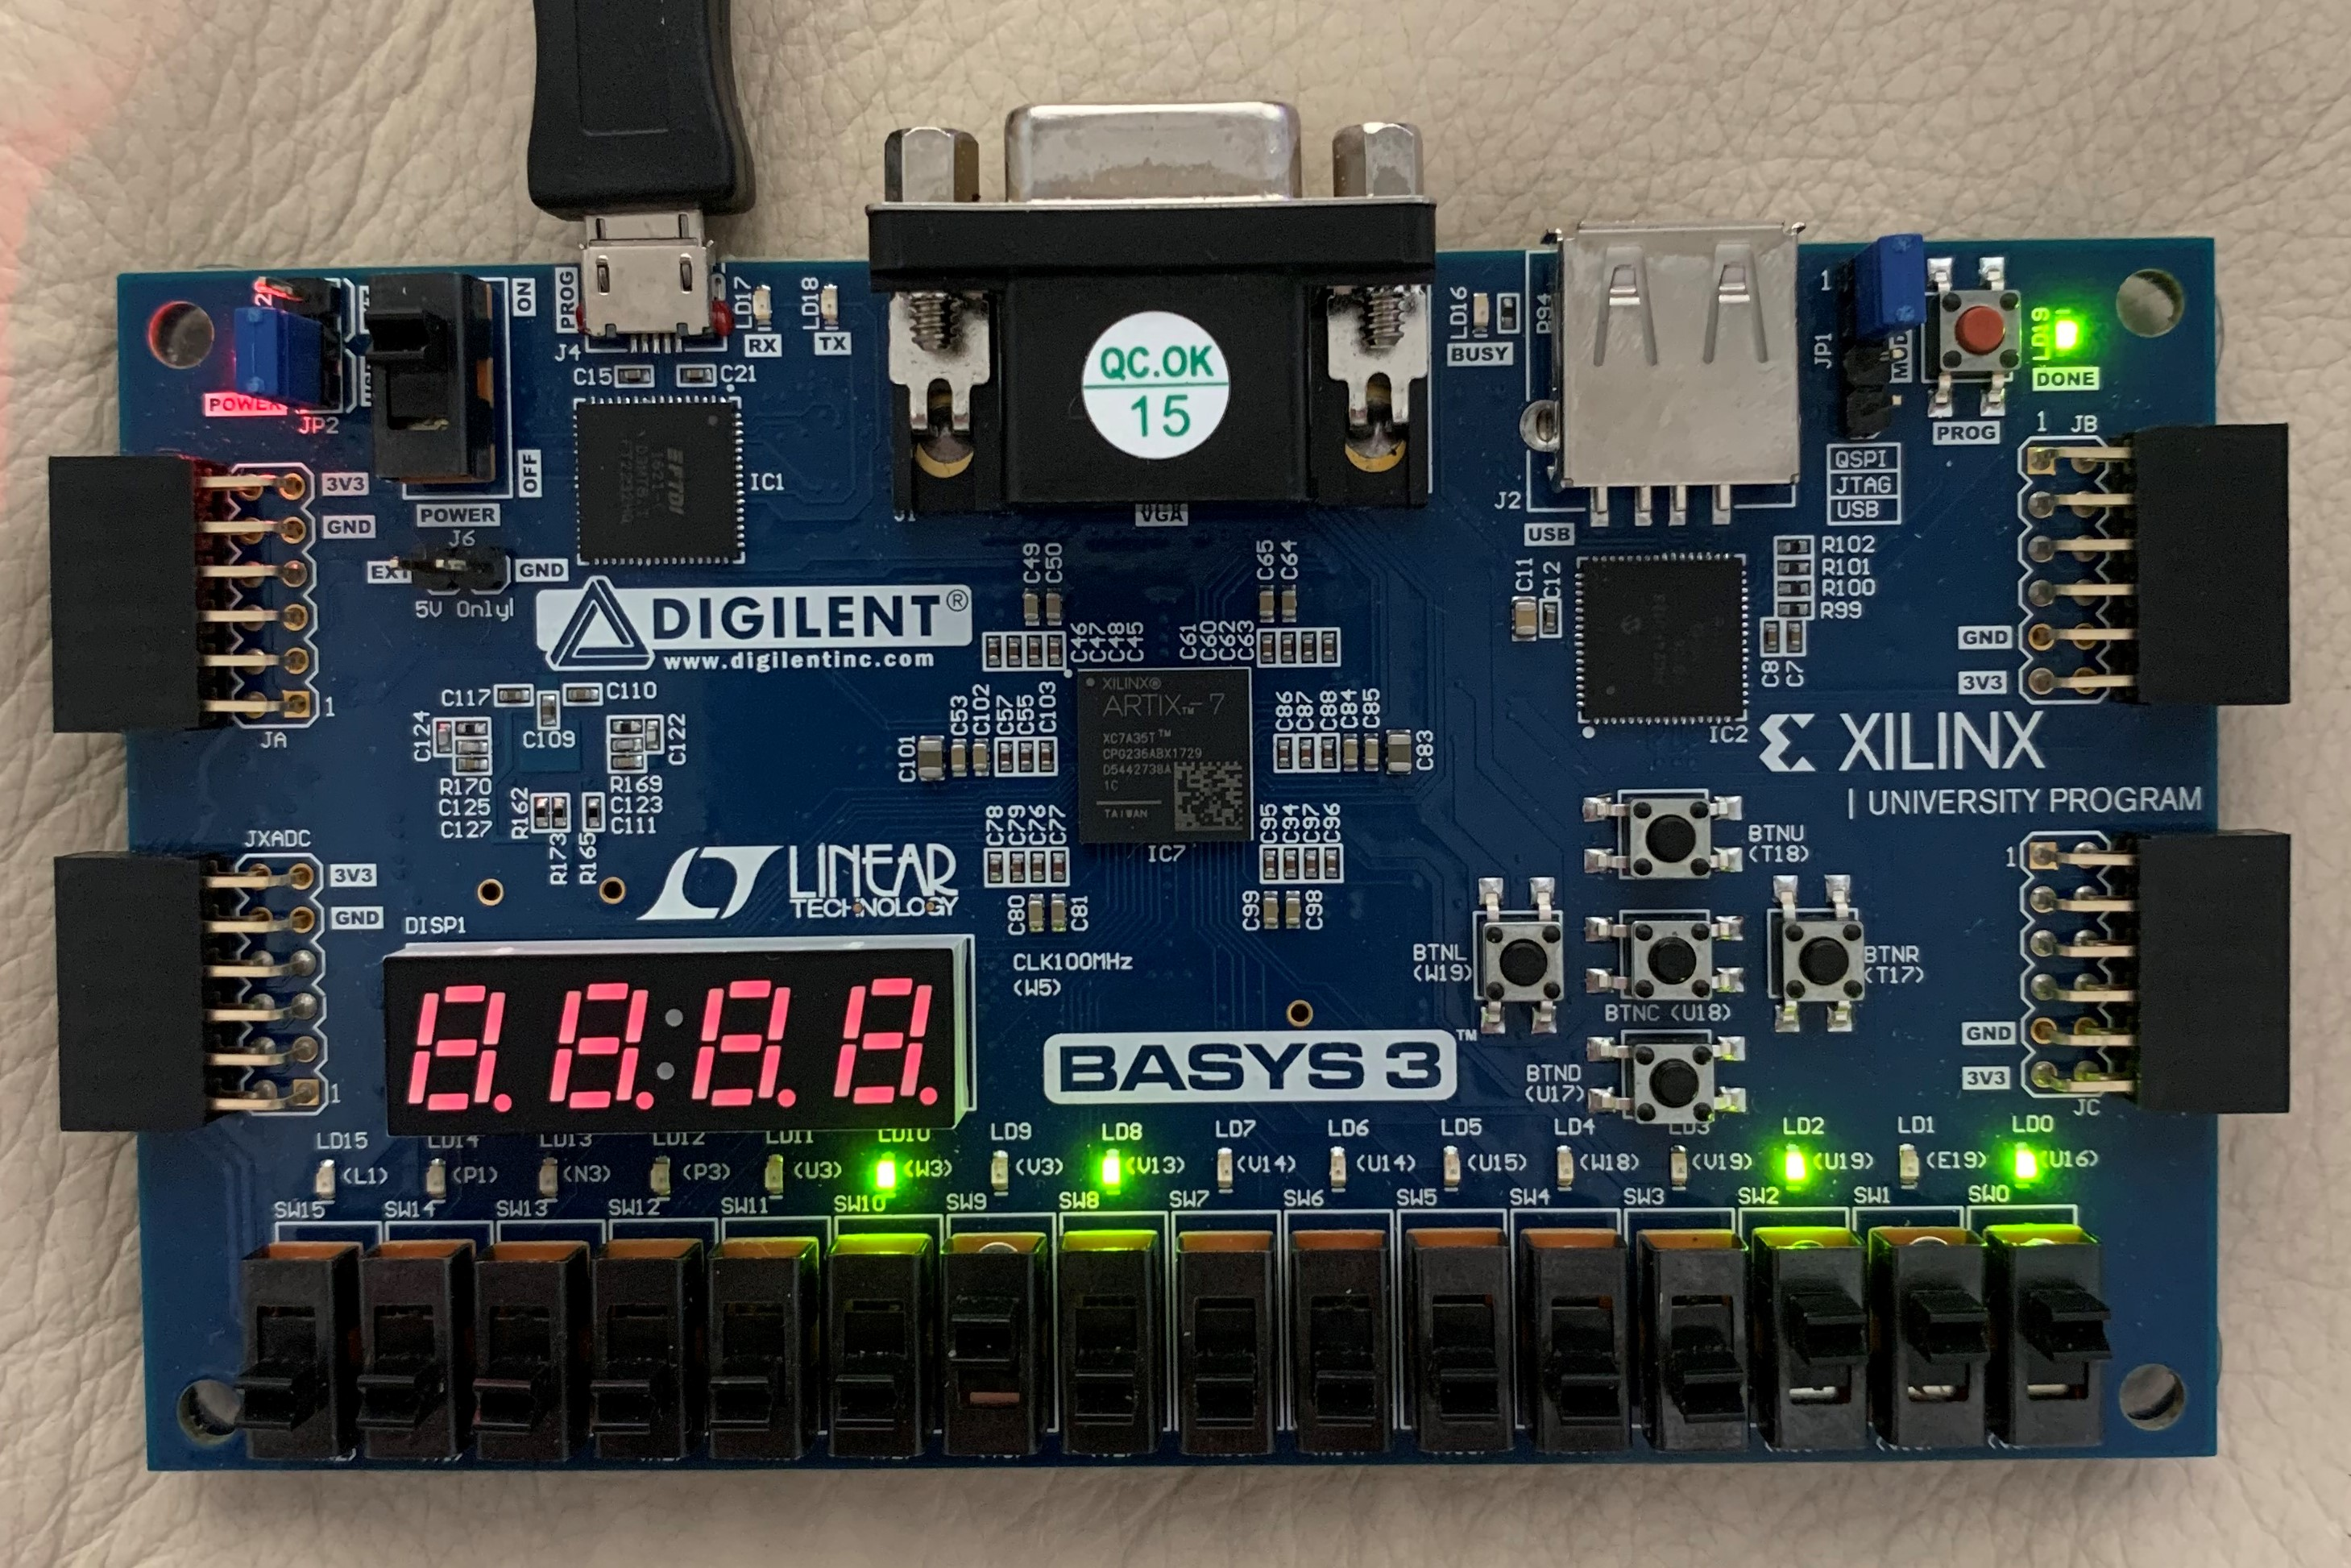
\includegraphics[width=0.8\textwidth,trim=0cm 0cm 0cm 0cm,clip]{and_step_2}
	\caption{Step 2 of AND (introduce 111 to get 101)}
	\label{fig:and_step_2}			
\end{figure}
\clearpage

\section*{Op 3: OR}

\begin{figure}[ht]\centering
	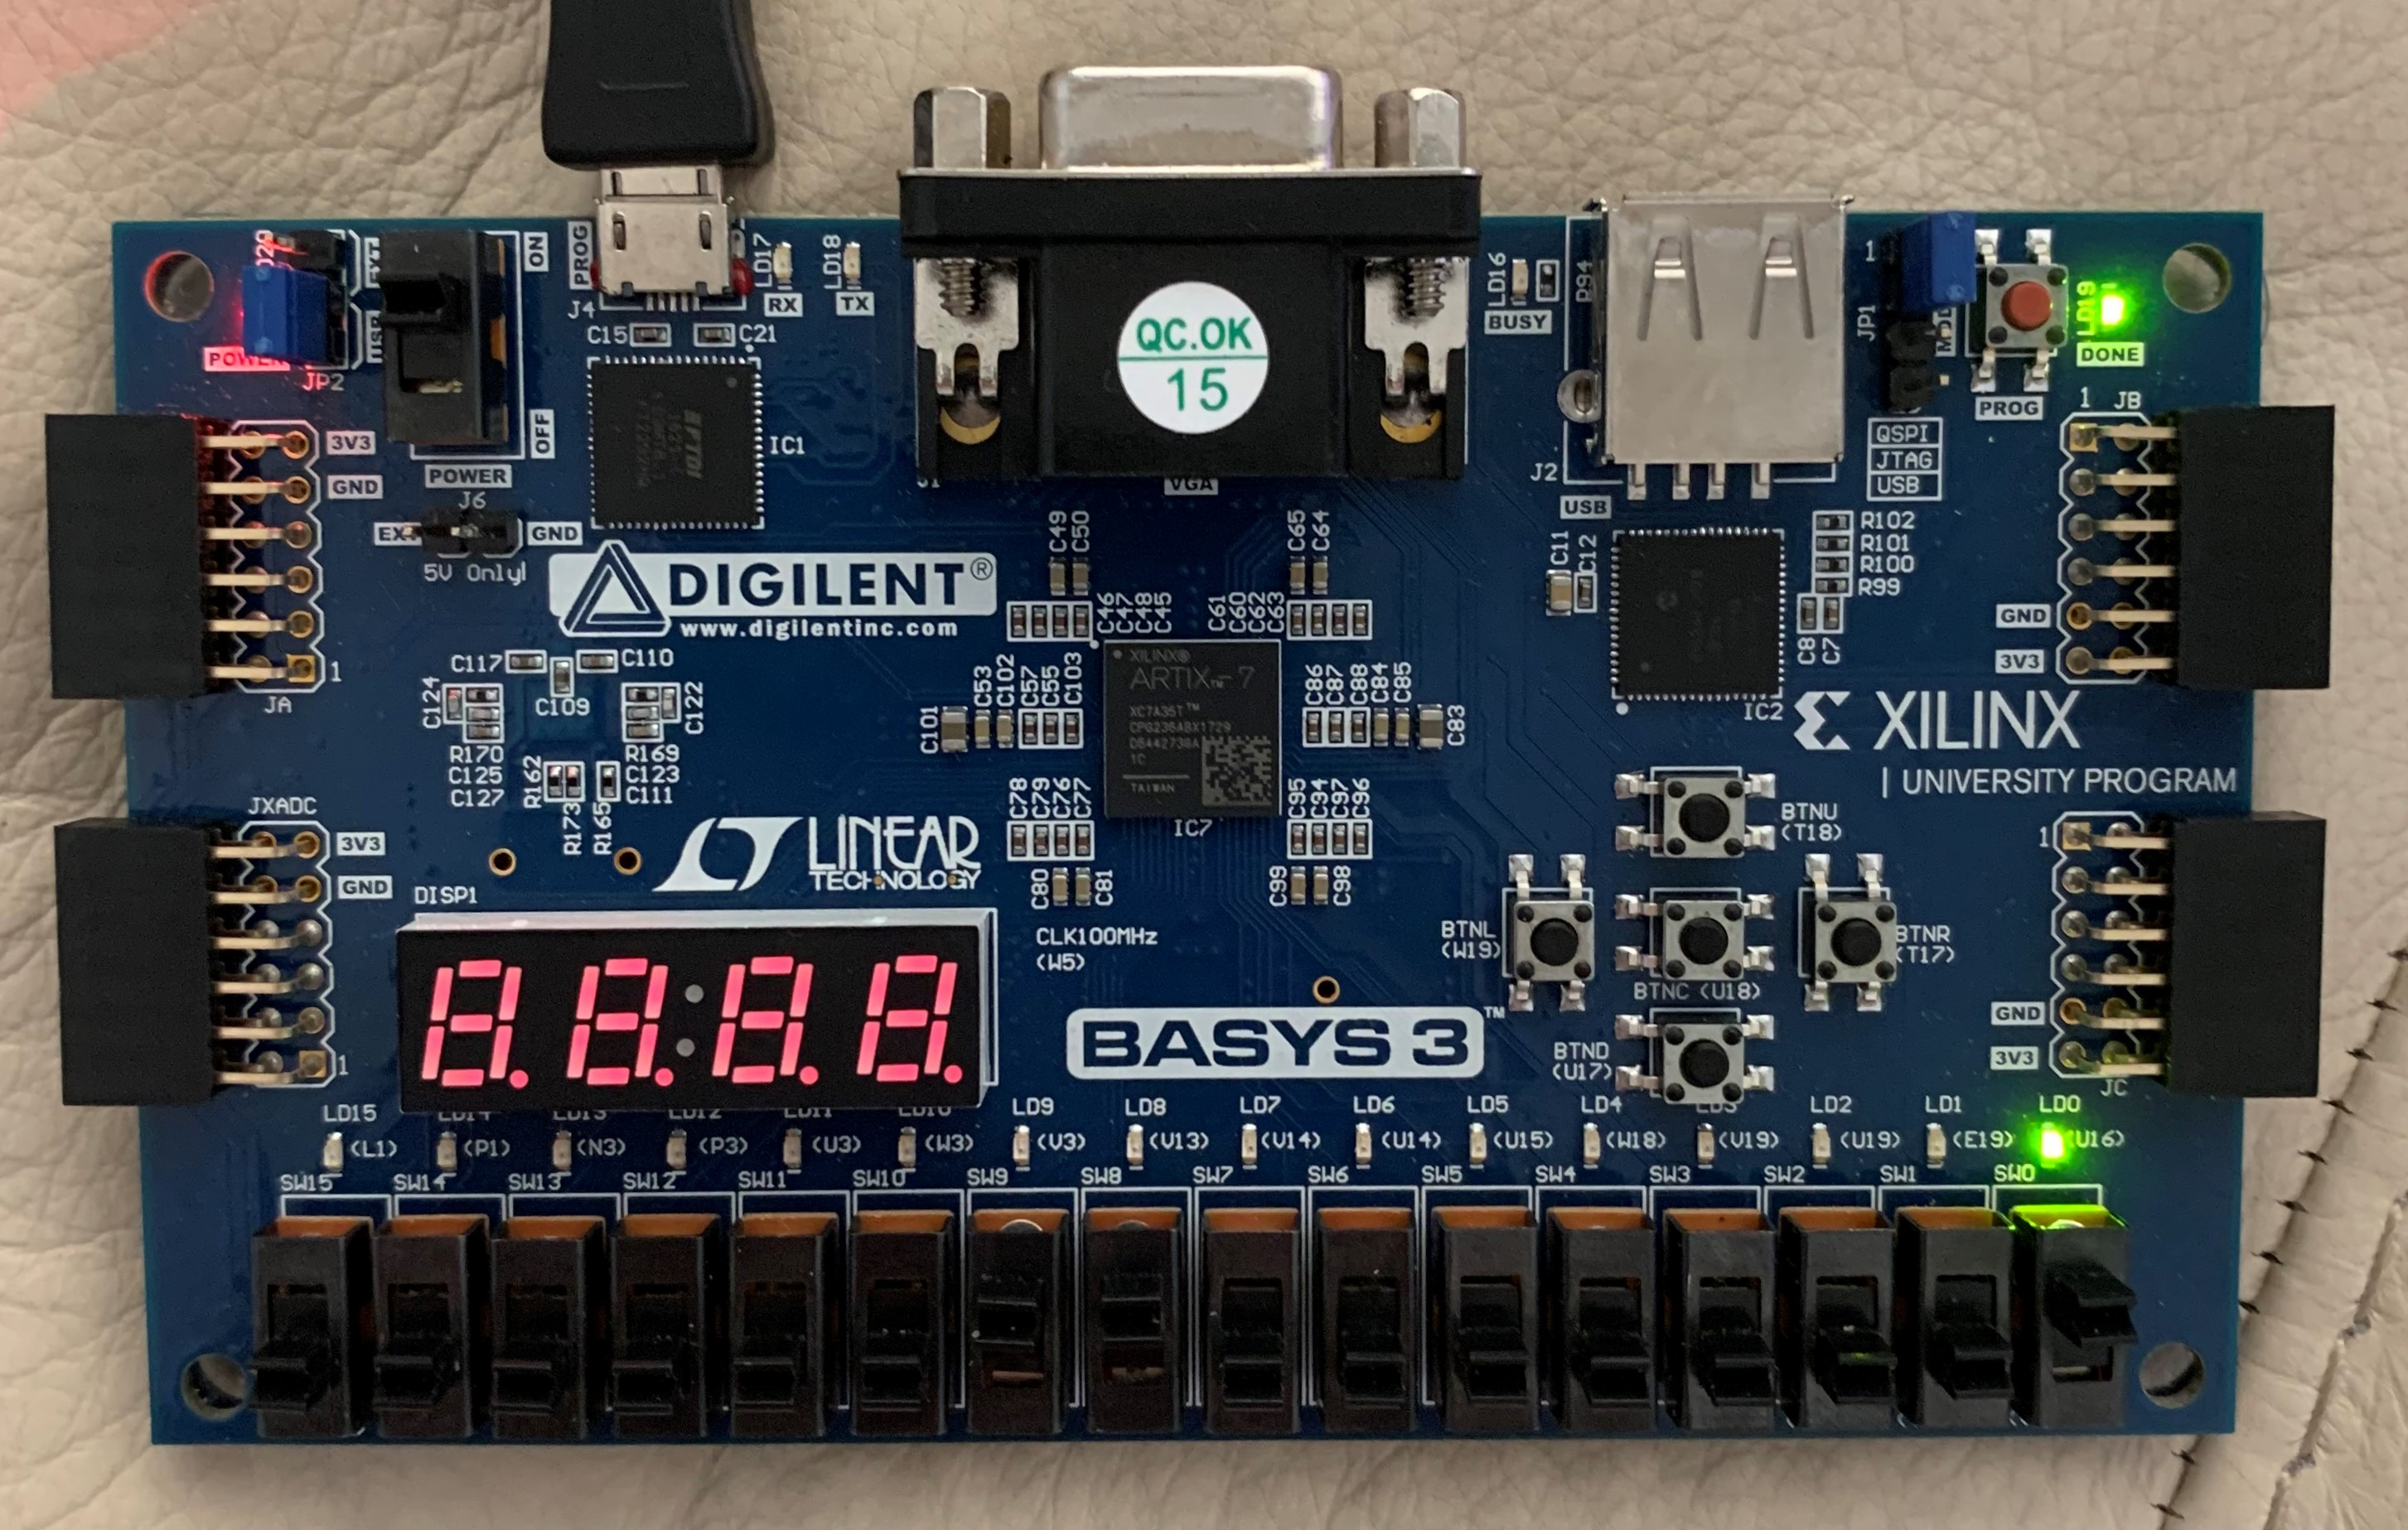
\includegraphics[width=0.8\textwidth,trim=0cm 0cm 0cm 0cm,clip]{or_step_1}
	\caption{Step 1 of OR (start with 1)}
	\label{fig:or_step_1}			
\end{figure}

\begin{figure}[ht]\centering
	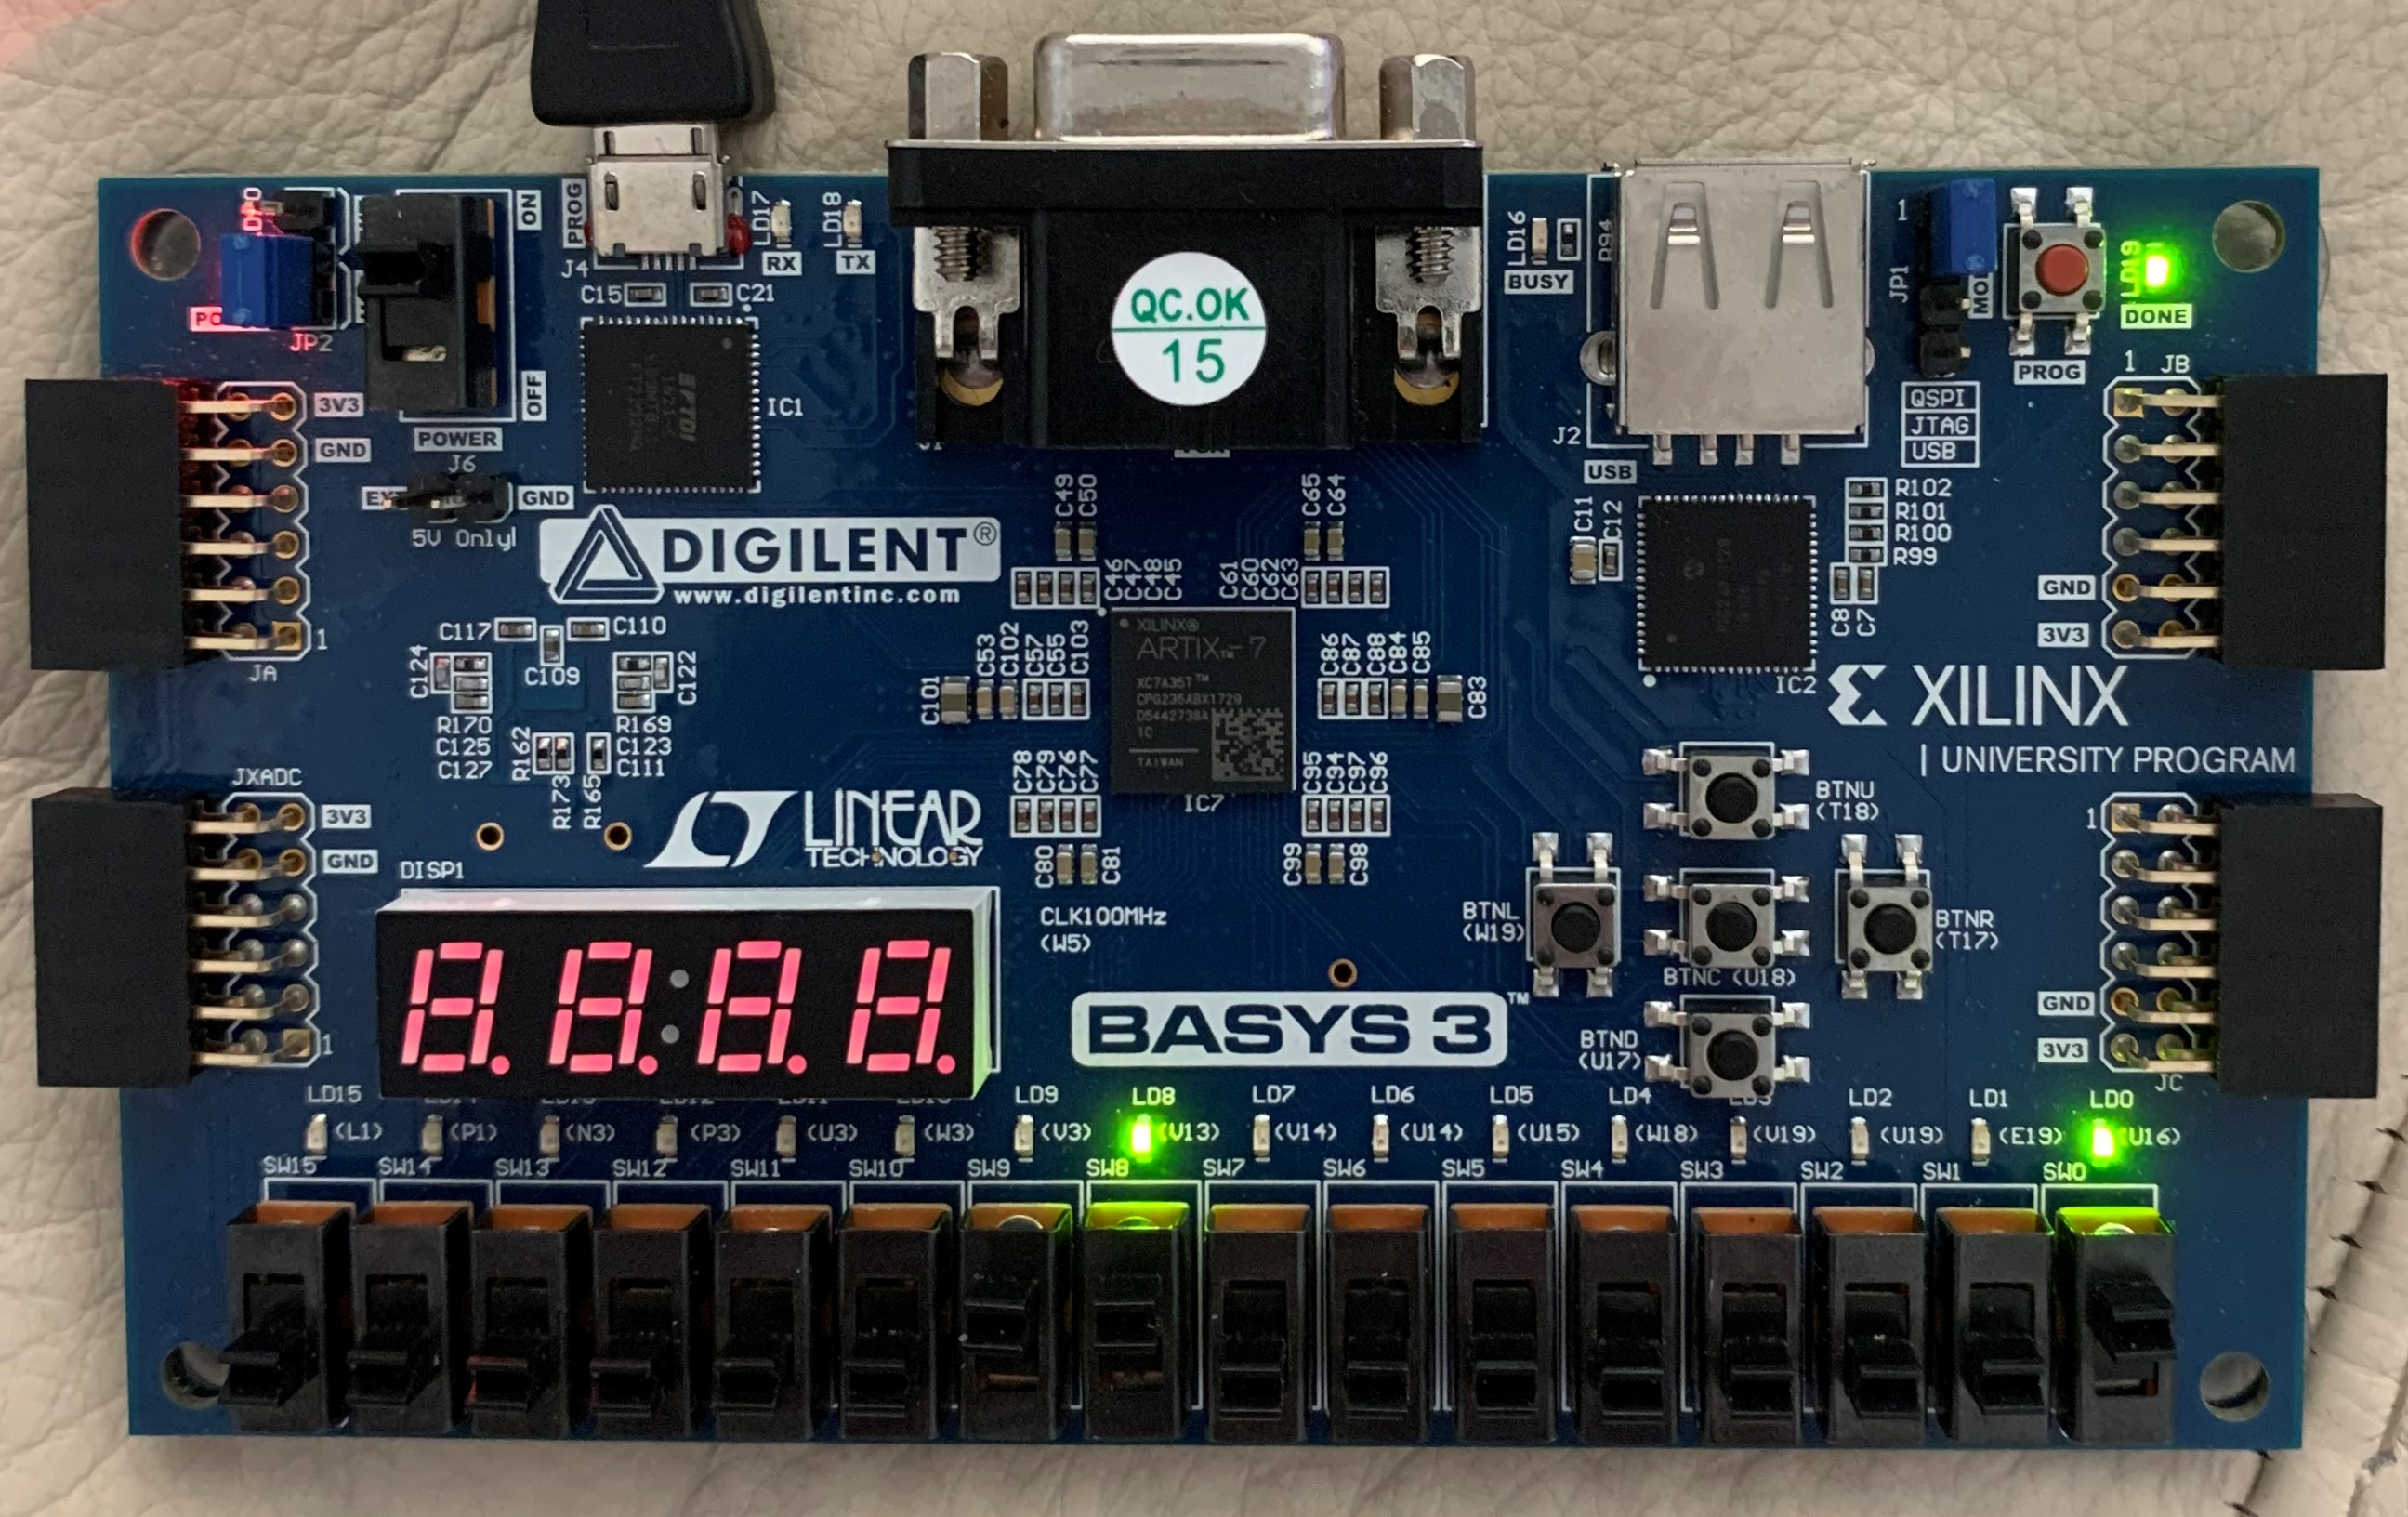
\includegraphics[width=0.8\textwidth,trim=0cm 0cm 0cm 0cm,clip]{or_step_2}
	\caption{Step 2 of OR (set)}
	\label{fig:or_step_2}			
\end{figure}

\begin{figure}[ht]\centering
	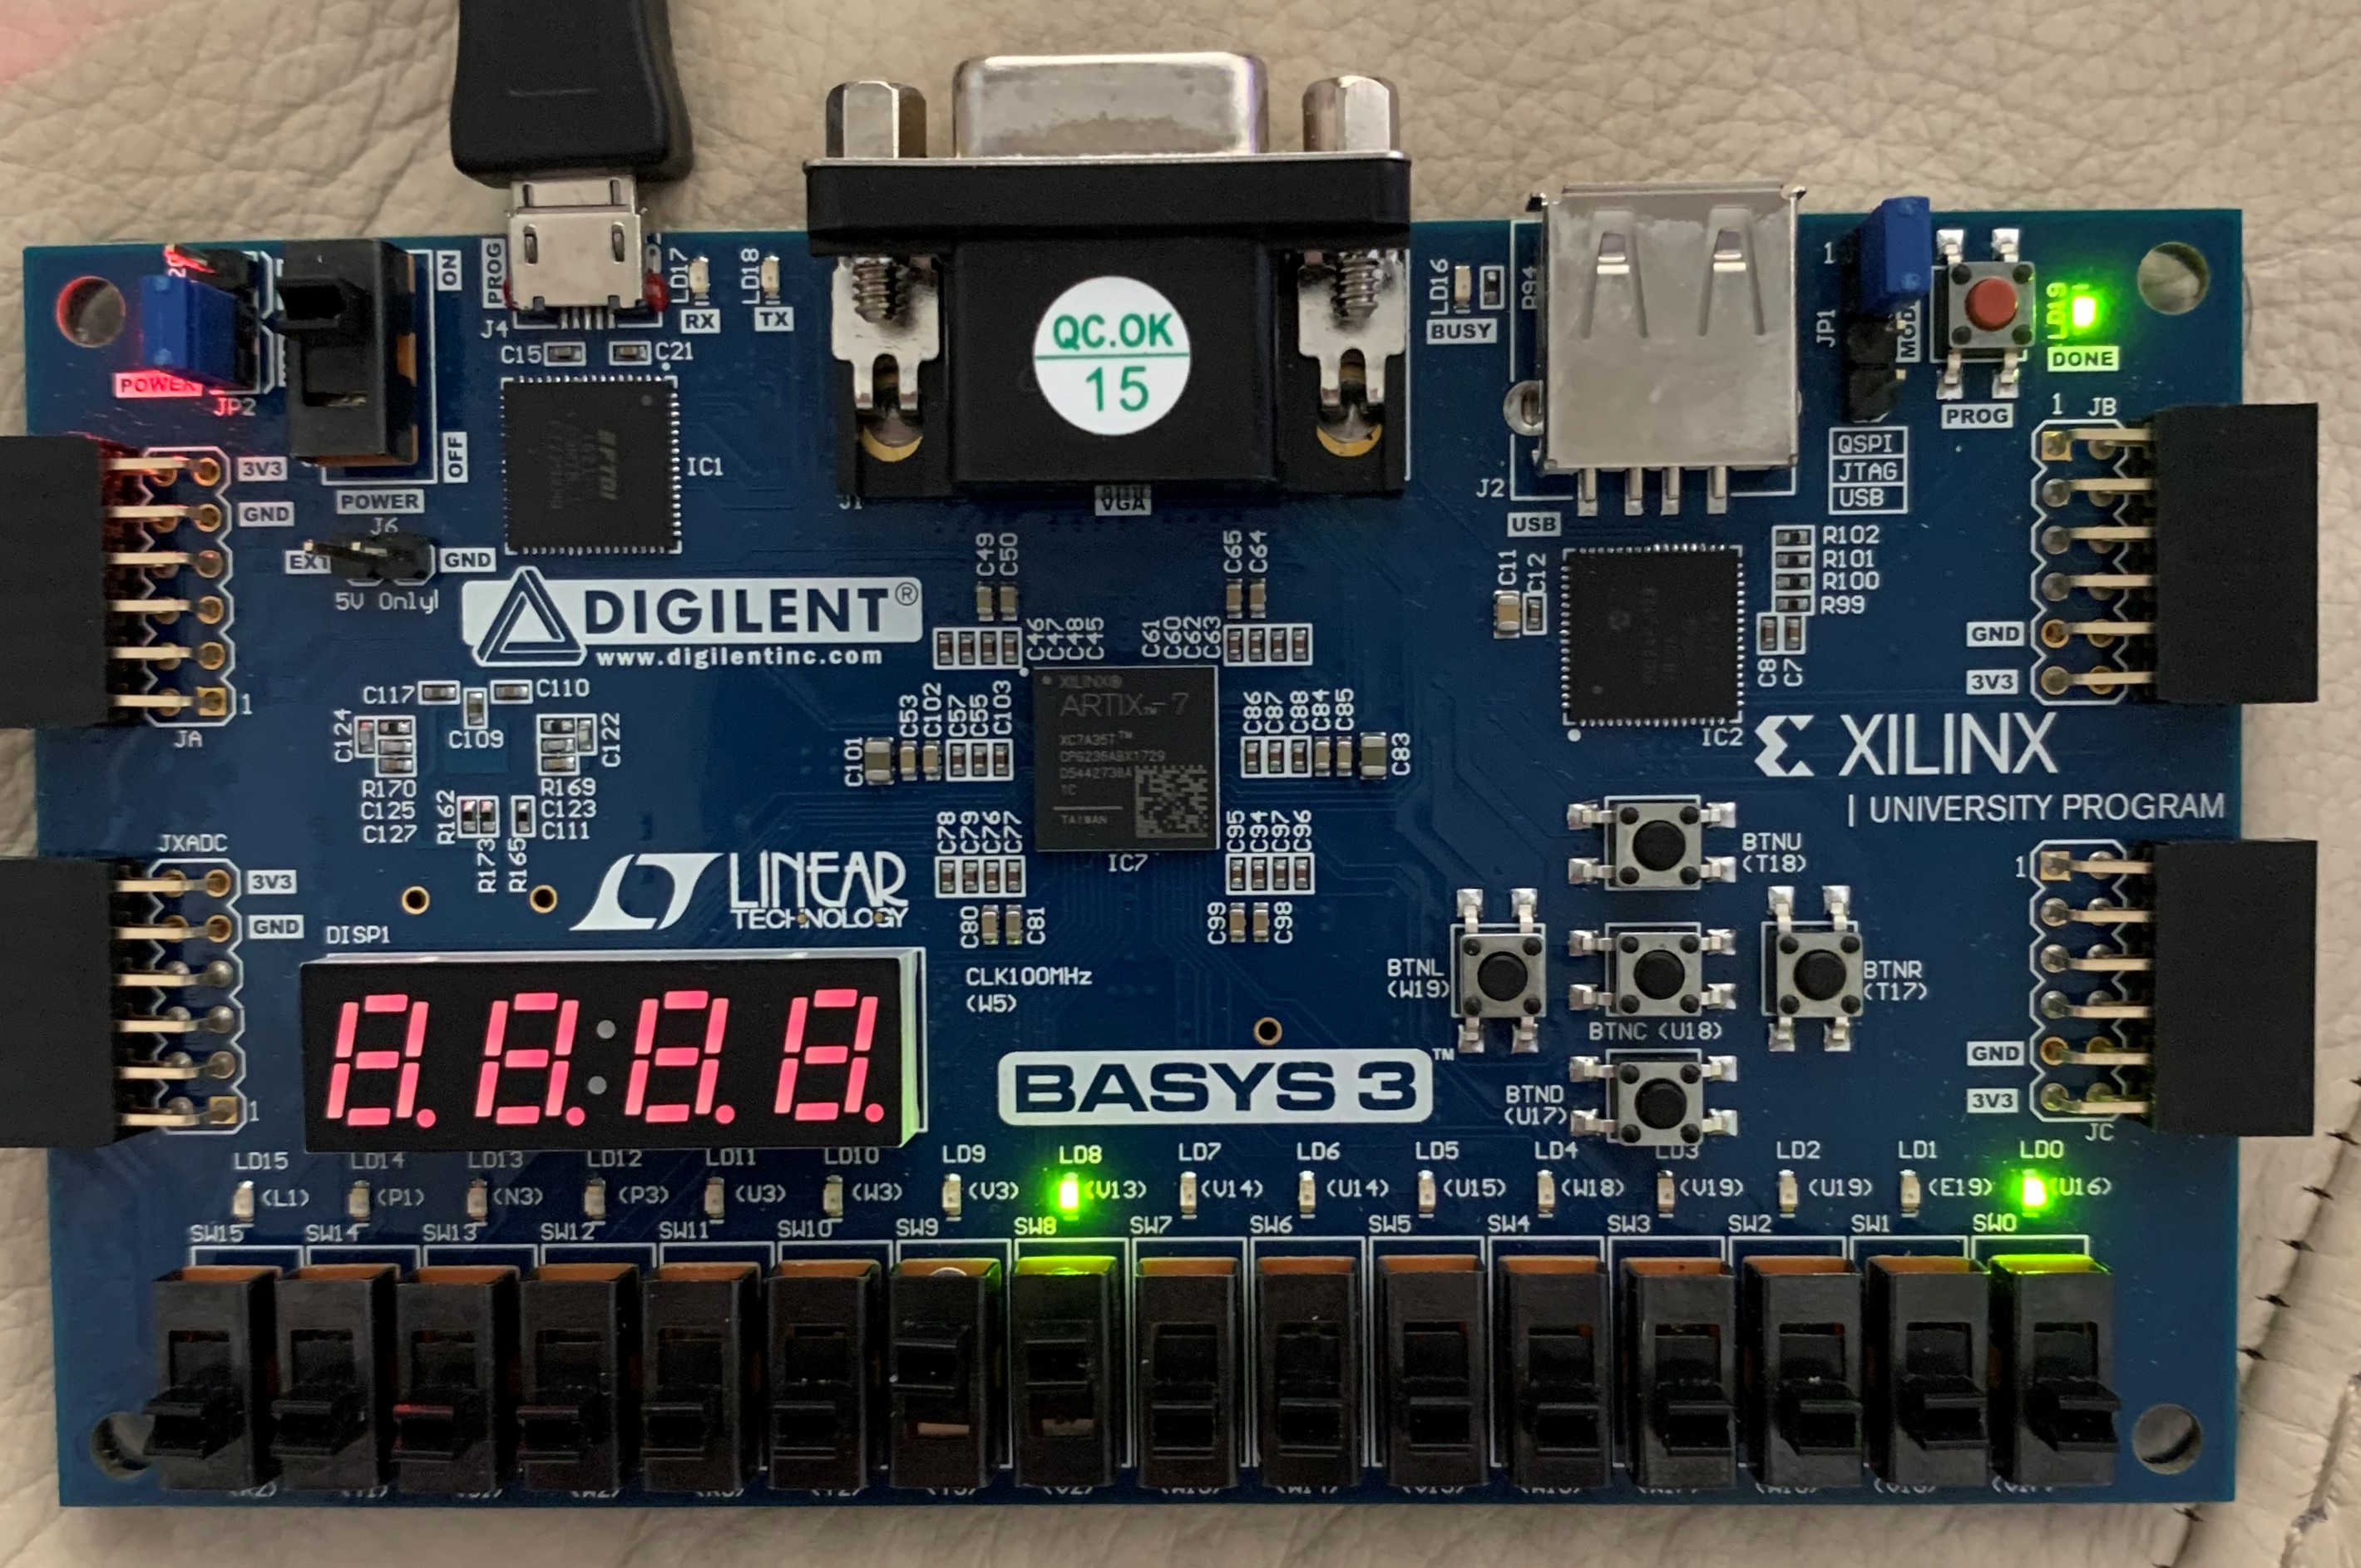
\includegraphics[width=0.8\textwidth,trim=0cm 0cm 0cm 0cm,clip]{or_step_3}
	\caption{Step 3 of OR (introduce 1 to get 1)}
	\label{fig:or_step_3}			
\end{figure}
\clearpage

\section*{Op 4: XOR}

\begin{figure}[ht]\centering
	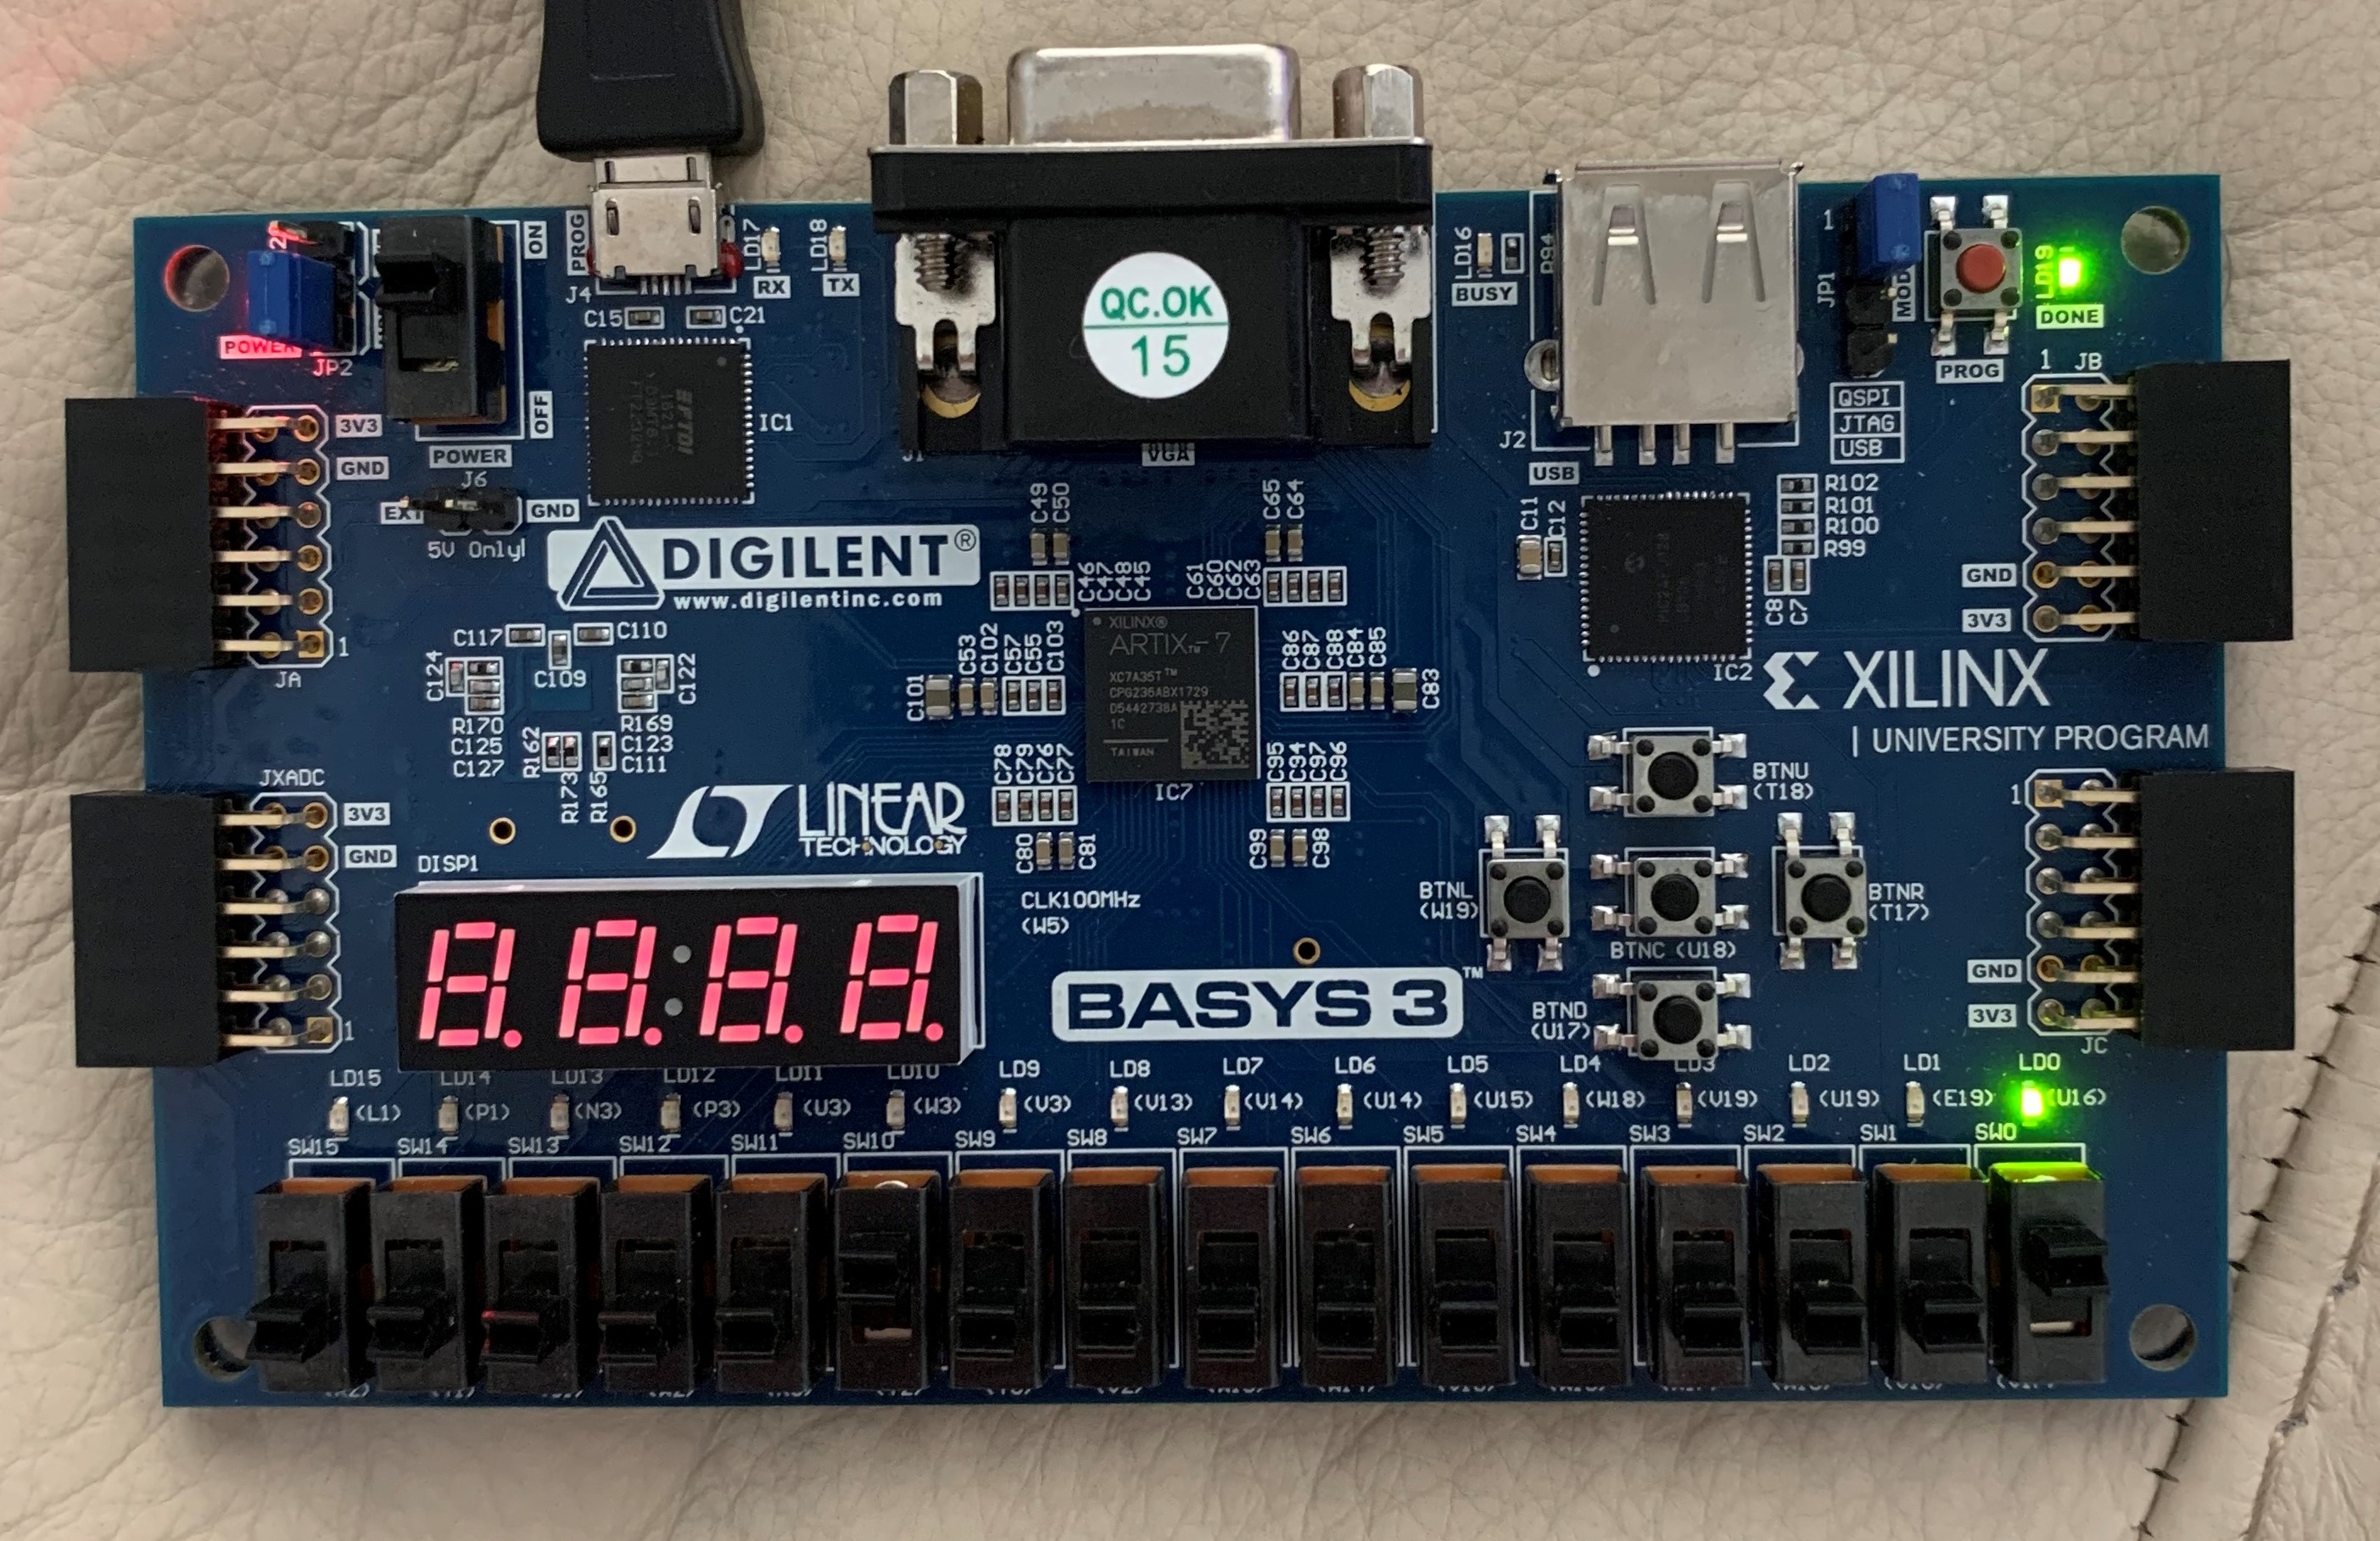
\includegraphics[width=0.8\textwidth,trim=0cm 0cm 0cm 0cm,clip]{xor_step_1}
	\caption{Step 1 of XOR (start with 1)}
	\label{fig:xor_step_1}			
\end{figure}

\begin{figure}[ht]\centering
	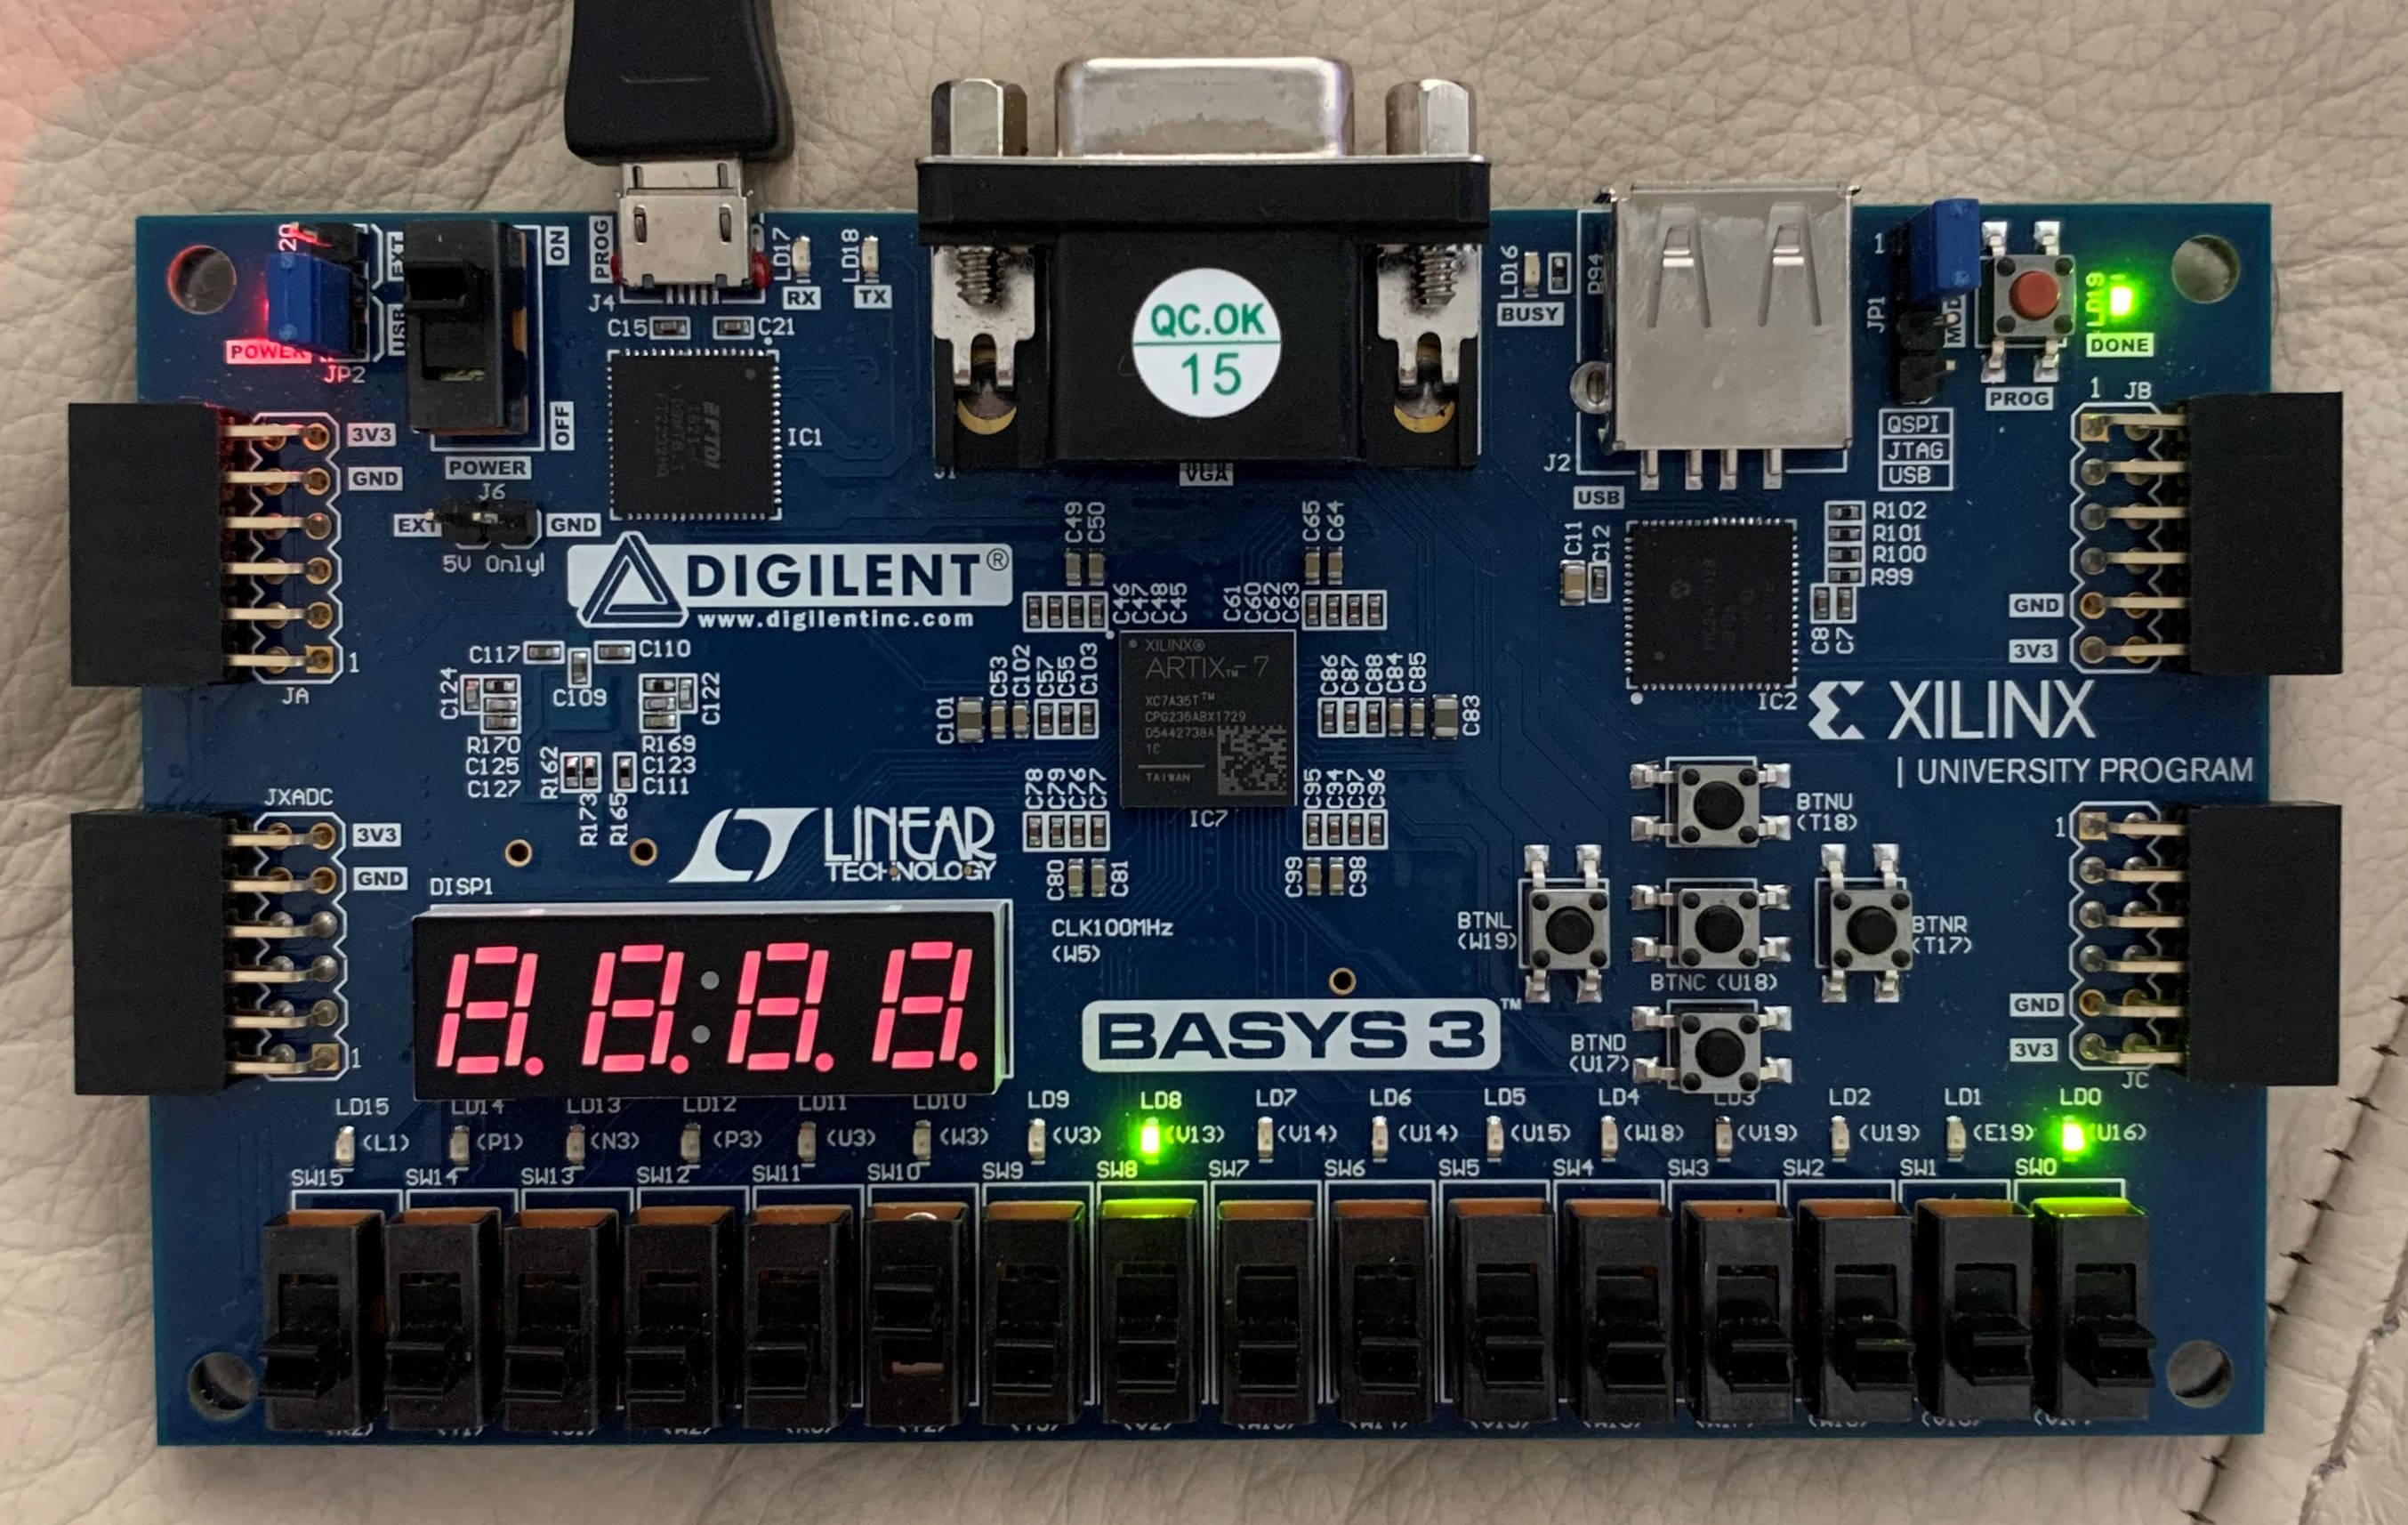
\includegraphics[width=0.8\textwidth,trim=0cm 0cm 0cm 0cm,clip]{xor_step_2}
	\caption{Step 2 of XOR (set)}
	\label{fig:xor_step_2}			
\end{figure}

\begin{figure}[ht]\centering
	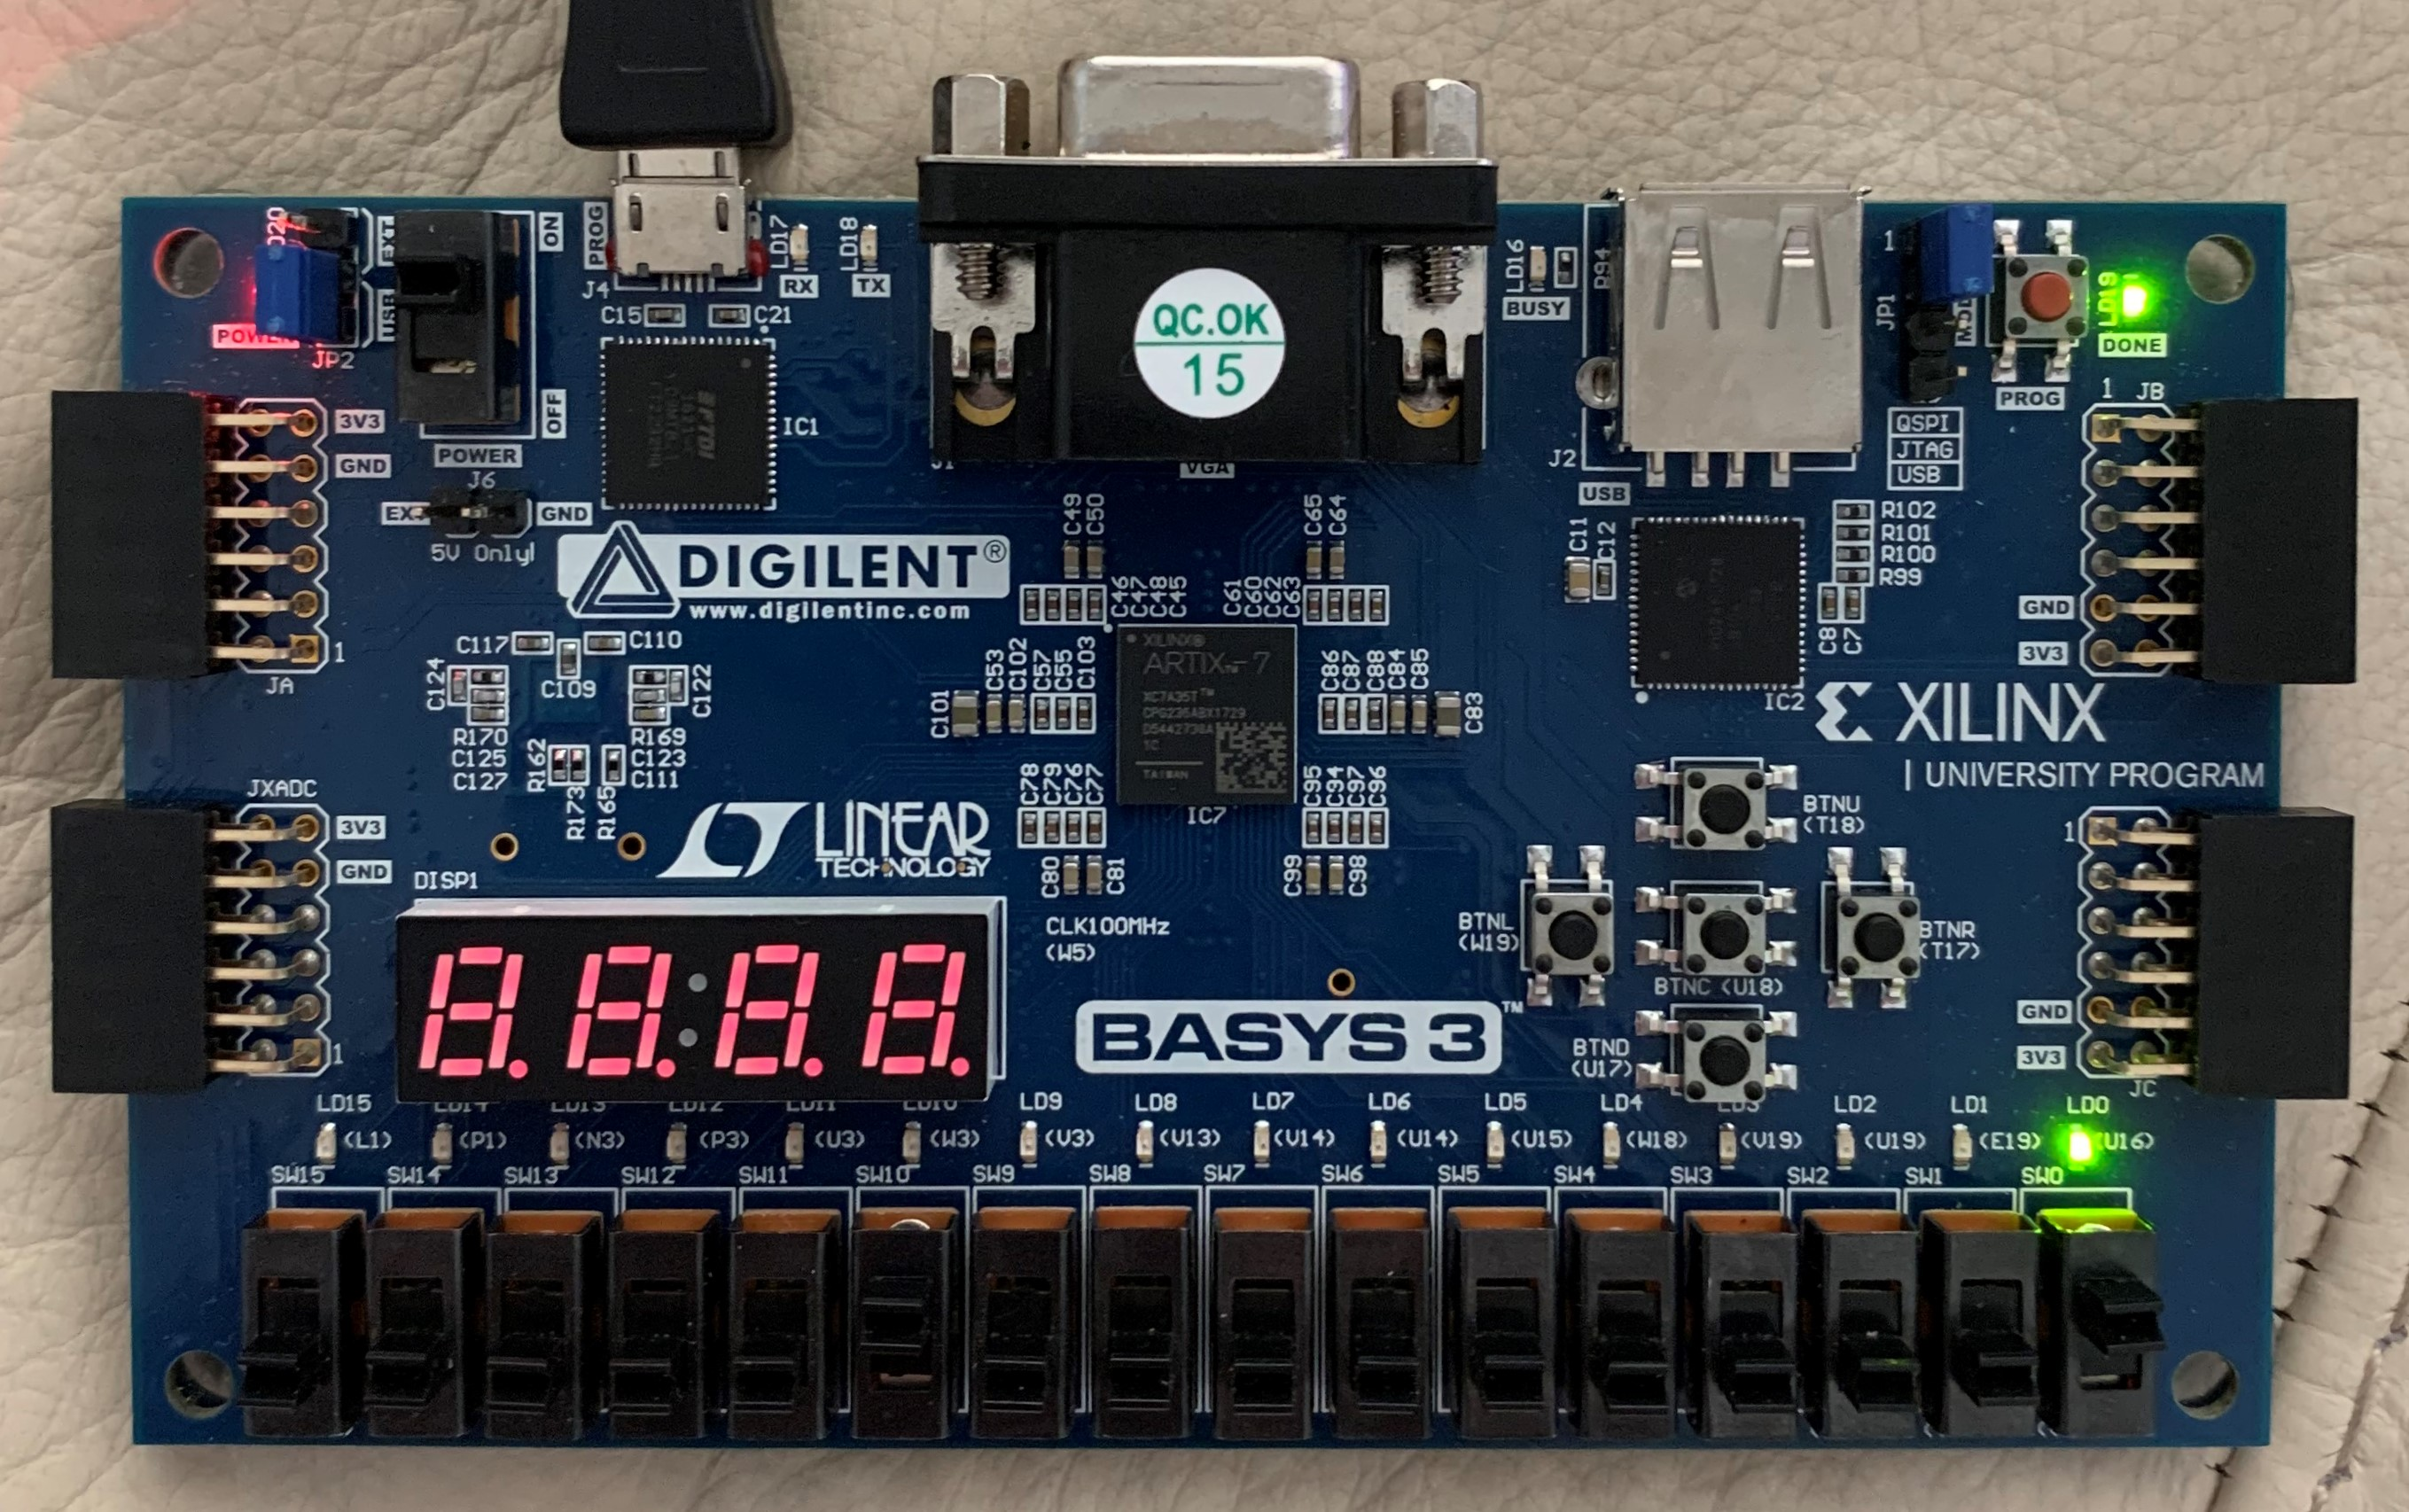
\includegraphics[width=0.8\textwidth,trim=0cm 0cm 0cm 0cm,clip]{xor_step_3}
	\caption{Step 3 of XOR (introduce 1 to get 0)}
	\label{fig:xor_step_3}			
\end{figure}
\clearpage
			
\section*{Code}

\Verilog[caption=Register Module,label=code:register]{register.sv}

\Verilog[caption=Register Test Bench,label=code:register_test]{register_test.sv}

\Verilog[caption=ALU Module,label=code:alu]{alu.sv}

\Verilog[caption=ALU Test Bench,label=code:alu_test]{alu_test.sv}

\Verilog[caption=Top Module,label=code:top_module]{top_lab9.sv}

\end{document}

